% Options for packages loaded elsewhere
\PassOptionsToPackage{unicode}{hyperref}
\PassOptionsToPackage{hyphens}{url}
%
\documentclass[
]{book}
\usepackage{lmodern}
\usepackage{amssymb,amsmath}
\usepackage{ifxetex,ifluatex}
\ifnum 0\ifxetex 1\fi\ifluatex 1\fi=0 % if pdftex
  \usepackage[T1]{fontenc}
  \usepackage[utf8]{inputenc}
  \usepackage{textcomp} % provide euro and other symbols
\else % if luatex or xetex
  \usepackage{unicode-math}
  \defaultfontfeatures{Scale=MatchLowercase}
  \defaultfontfeatures[\rmfamily]{Ligatures=TeX,Scale=1}
\fi
% Use upquote if available, for straight quotes in verbatim environments
\IfFileExists{upquote.sty}{\usepackage{upquote}}{}
\IfFileExists{microtype.sty}{% use microtype if available
  \usepackage[]{microtype}
  \UseMicrotypeSet[protrusion]{basicmath} % disable protrusion for tt fonts
}{}
\makeatletter
\@ifundefined{KOMAClassName}{% if non-KOMA class
  \IfFileExists{parskip.sty}{%
    \usepackage{parskip}
  }{% else
    \setlength{\parindent}{0pt}
    \setlength{\parskip}{6pt plus 2pt minus 1pt}}
}{% if KOMA class
  \KOMAoptions{parskip=half}}
\makeatother
\usepackage{xcolor}
\IfFileExists{xurl.sty}{\usepackage{xurl}}{} % add URL line breaks if available
\IfFileExists{bookmark.sty}{\usepackage{bookmark}}{\usepackage{hyperref}}
\hypersetup{
  pdftitle={Correlation and Regression},
  pdfauthor={Seth Harrison},
  hidelinks,
  pdfcreator={LaTeX via pandoc}}
\urlstyle{same} % disable monospaced font for URLs
\usepackage{color}
\usepackage{fancyvrb}
\newcommand{\VerbBar}{|}
\newcommand{\VERB}{\Verb[commandchars=\\\{\}]}
\DefineVerbatimEnvironment{Highlighting}{Verbatim}{commandchars=\\\{\}}
% Add ',fontsize=\small' for more characters per line
\usepackage{framed}
\definecolor{shadecolor}{RGB}{248,248,248}
\newenvironment{Shaded}{\begin{snugshade}}{\end{snugshade}}
\newcommand{\AlertTok}[1]{\textcolor[rgb]{0.94,0.16,0.16}{#1}}
\newcommand{\AnnotationTok}[1]{\textcolor[rgb]{0.56,0.35,0.01}{\textbf{\textit{#1}}}}
\newcommand{\AttributeTok}[1]{\textcolor[rgb]{0.77,0.63,0.00}{#1}}
\newcommand{\BaseNTok}[1]{\textcolor[rgb]{0.00,0.00,0.81}{#1}}
\newcommand{\BuiltInTok}[1]{#1}
\newcommand{\CharTok}[1]{\textcolor[rgb]{0.31,0.60,0.02}{#1}}
\newcommand{\CommentTok}[1]{\textcolor[rgb]{0.56,0.35,0.01}{\textit{#1}}}
\newcommand{\CommentVarTok}[1]{\textcolor[rgb]{0.56,0.35,0.01}{\textbf{\textit{#1}}}}
\newcommand{\ConstantTok}[1]{\textcolor[rgb]{0.00,0.00,0.00}{#1}}
\newcommand{\ControlFlowTok}[1]{\textcolor[rgb]{0.13,0.29,0.53}{\textbf{#1}}}
\newcommand{\DataTypeTok}[1]{\textcolor[rgb]{0.13,0.29,0.53}{#1}}
\newcommand{\DecValTok}[1]{\textcolor[rgb]{0.00,0.00,0.81}{#1}}
\newcommand{\DocumentationTok}[1]{\textcolor[rgb]{0.56,0.35,0.01}{\textbf{\textit{#1}}}}
\newcommand{\ErrorTok}[1]{\textcolor[rgb]{0.64,0.00,0.00}{\textbf{#1}}}
\newcommand{\ExtensionTok}[1]{#1}
\newcommand{\FloatTok}[1]{\textcolor[rgb]{0.00,0.00,0.81}{#1}}
\newcommand{\FunctionTok}[1]{\textcolor[rgb]{0.00,0.00,0.00}{#1}}
\newcommand{\ImportTok}[1]{#1}
\newcommand{\InformationTok}[1]{\textcolor[rgb]{0.56,0.35,0.01}{\textbf{\textit{#1}}}}
\newcommand{\KeywordTok}[1]{\textcolor[rgb]{0.13,0.29,0.53}{\textbf{#1}}}
\newcommand{\NormalTok}[1]{#1}
\newcommand{\OperatorTok}[1]{\textcolor[rgb]{0.81,0.36,0.00}{\textbf{#1}}}
\newcommand{\OtherTok}[1]{\textcolor[rgb]{0.56,0.35,0.01}{#1}}
\newcommand{\PreprocessorTok}[1]{\textcolor[rgb]{0.56,0.35,0.01}{\textit{#1}}}
\newcommand{\RegionMarkerTok}[1]{#1}
\newcommand{\SpecialCharTok}[1]{\textcolor[rgb]{0.00,0.00,0.00}{#1}}
\newcommand{\SpecialStringTok}[1]{\textcolor[rgb]{0.31,0.60,0.02}{#1}}
\newcommand{\StringTok}[1]{\textcolor[rgb]{0.31,0.60,0.02}{#1}}
\newcommand{\VariableTok}[1]{\textcolor[rgb]{0.00,0.00,0.00}{#1}}
\newcommand{\VerbatimStringTok}[1]{\textcolor[rgb]{0.31,0.60,0.02}{#1}}
\newcommand{\WarningTok}[1]{\textcolor[rgb]{0.56,0.35,0.01}{\textbf{\textit{#1}}}}
\usepackage{longtable,booktabs}
% Correct order of tables after \paragraph or \subparagraph
\usepackage{etoolbox}
\makeatletter
\patchcmd\longtable{\par}{\if@noskipsec\mbox{}\fi\par}{}{}
\makeatother
% Allow footnotes in longtable head/foot
\IfFileExists{footnotehyper.sty}{\usepackage{footnotehyper}}{\usepackage{footnote}}
\makesavenoteenv{longtable}
\usepackage{graphicx,grffile}
\makeatletter
\def\maxwidth{\ifdim\Gin@nat@width>\linewidth\linewidth\else\Gin@nat@width\fi}
\def\maxheight{\ifdim\Gin@nat@height>\textheight\textheight\else\Gin@nat@height\fi}
\makeatother
% Scale images if necessary, so that they will not overflow the page
% margins by default, and it is still possible to overwrite the defaults
% using explicit options in \includegraphics[width, height, ...]{}
\setkeys{Gin}{width=\maxwidth,height=\maxheight,keepaspectratio}
% Set default figure placement to htbp
\makeatletter
\def\fps@figure{htbp}
\makeatother
\setlength{\emergencystretch}{3em} % prevent overfull lines
\providecommand{\tightlist}{%
  \setlength{\itemsep}{0pt}\setlength{\parskip}{0pt}}
\setcounter{secnumdepth}{5}
\usepackage{booktabs}
\usepackage[]{natbib}
\bibliographystyle{apalike}

\title{\href{https://www.datacamp.com/courses/correlation-and-regression}{Correlation and Regression}}
\author{\href{https://username.github.io/}{Seth Harrison}}
\date{Last compiled: Feb 12, 2021}

\begin{document}
\maketitle

{
\setcounter{tocdepth}{1}
\tableofcontents
}
\hypertarget{prerequisites}{%
\chapter{Prerequisites}\label{prerequisites}}

This material is from the \href{https://www.datacamp.com}{DataCamp} course \href{https://www.datacamp.com/courses/correlation-and-regression}{Correlation and Regression} by Ben Baumer. Before using this material, the reader should have completed and be comfortable with the material in the DataCamp modules \href{https://www.datacamp.com/courses/free-introduction-to-r}{Introduction to R}.

Reminder to self: each \texttt{*.Rmd} file contains one and only one chapter, and a chapter is defined by the first-level heading \texttt{\#}.

\hypertarget{visualizing-two-variables}{%
\chapter{Visualizing two variables}\label{visualizing-two-variables}}

In this chapter, you will learn techniques for exploring bivariate relationships.

\begin{center}\rule{0.5\linewidth}{0.5pt}\end{center}

\begin{center}\rule{0.5\linewidth}{0.5pt}\end{center}

\hypertarget{scatterplots}{%
\section{Scatterplots}\label{scatterplots}}

Scatterplots are the most common and effective tools for visualizing the relationship between two numeric variables.

The \texttt{ncbirths} dataset is a random sample of 1,000 cases taken from a larger dataset collected in 2004. Each case describes the birth of a single child born in North Carolina, along with various characteristics of the child (e.g.~birth weight, length of gestation, etc.), the child's mother (e.g.~age, weight gained during pregnancy, smoking habits, etc.) and the child's father (e.g.~age). You can view the help file for these data by running \texttt{?ncbirths} in the console.

\begin{Shaded}
\begin{Highlighting}[]
\KeywordTok{library}\NormalTok{(openintro)}
\NormalTok{DT}\OperatorTok{::}\KeywordTok{datatable}\NormalTok{(ncbirths)}
\end{Highlighting}
\end{Shaded}

\begin{verbatim}
PhantomJS not found. You can install it with webshot::install_phantomjs(). If it is installed, please make sure the phantomjs executable can be found via the PATH variable.
\end{verbatim}

\begin{center}\rule{0.5\linewidth}{0.5pt}\end{center}

\hypertarget{exercise}{%
\subsection*{Exercise}\label{exercise}}
\addcontentsline{toc}{subsection}{Exercise}

Using the \texttt{ncbirths} dataset, make a scatterplot using \texttt{ggplot()} to illustrate how the birth weight of these babies varies according to the number of weeks of gestation.

\begin{Shaded}
\begin{Highlighting}[]
\CommentTok{# Scatterplot of weight vs. weeks}
\KeywordTok{library}\NormalTok{(ggplot2)}
\KeywordTok{ggplot}\NormalTok{(}\DataTypeTok{data =}\NormalTok{ ncbirths, }\KeywordTok{aes}\NormalTok{(}\DataTypeTok{y =}\NormalTok{ weight, }\DataTypeTok{x =}\NormalTok{ weeks)) }\OperatorTok{+}
\StringTok{  }\KeywordTok{geom_point}\NormalTok{(}\DataTypeTok{alpha =} \FloatTok{0.2}\NormalTok{) }\OperatorTok{+}\StringTok{ }
\StringTok{  }\KeywordTok{theme_bw}\NormalTok{()}
\end{Highlighting}
\end{Shaded}

\begin{verbatim}
Warning: Removed 2 rows containing missing values (geom_point).
\end{verbatim}

\begin{center}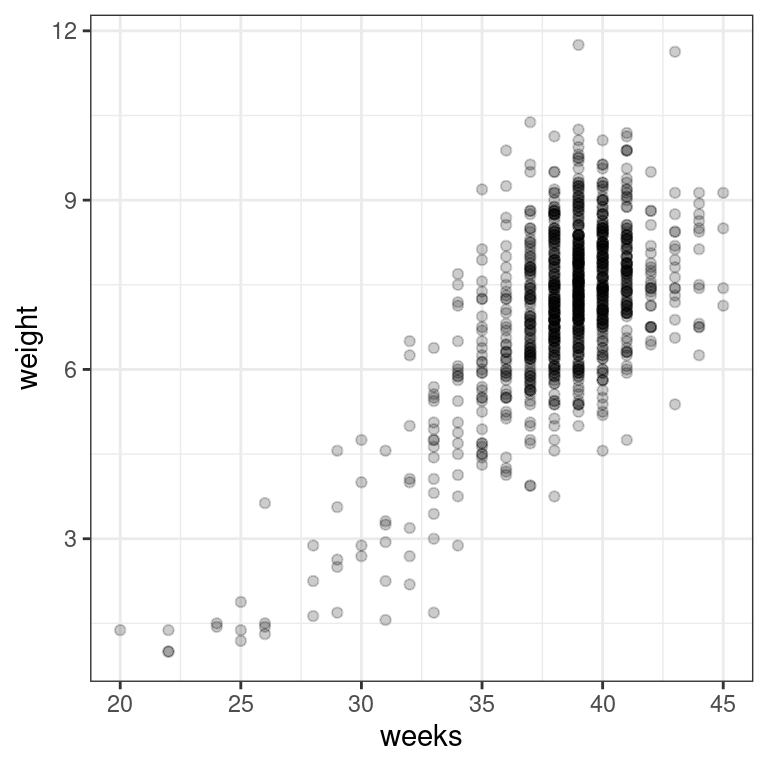
\includegraphics{CorrRegSC_files/figure-latex/unnamed-chunk-3-1} \end{center}

\begin{center}\rule{0.5\linewidth}{0.5pt}\end{center}

\hypertarget{boxplots-as-discretizedconditioned-scatterplots}{%
\section{Boxplots as discretized/conditioned scatterplots}\label{boxplots-as-discretizedconditioned-scatterplots}}

If it is helpful, you can think of boxplots as scatterplots for which the variable on the x-axis has been discretized.

The \texttt{cut()} function takes two arguments: the continuous variable you want to discretize and the number of \texttt{breaks} that you want to make in that continuous variable in order to discretize it.

\begin{center}\rule{0.5\linewidth}{0.5pt}\end{center}

\hypertarget{exercise-1}{%
\subsection*{Exercise}\label{exercise-1}}
\addcontentsline{toc}{subsection}{Exercise}

Using the \texttt{ncbirths} dataset again, make a boxplot illustrating how the birth weight of these babies varies according to the number of weeks of gestation. This time, use the \texttt{cut()} function to discretize the x-variable into six intervals (i.e.~five breaks).

\begin{Shaded}
\begin{Highlighting}[]
\CommentTok{# Boxplot of weight vs. weeks}
\KeywordTok{ggplot}\NormalTok{(}\DataTypeTok{data =}\NormalTok{ ncbirths, }
       \KeywordTok{aes}\NormalTok{(}\DataTypeTok{x =} \KeywordTok{cut}\NormalTok{(weeks, }\DataTypeTok{breaks =} \DecValTok{5}\NormalTok{), }\DataTypeTok{y =}\NormalTok{ weight)) }\OperatorTok{+}\StringTok{ }
\StringTok{       }\KeywordTok{geom_boxplot}\NormalTok{() }\OperatorTok{+}\StringTok{ }
\StringTok{       }\KeywordTok{theme_bw}\NormalTok{()}
\end{Highlighting}
\end{Shaded}

\begin{center}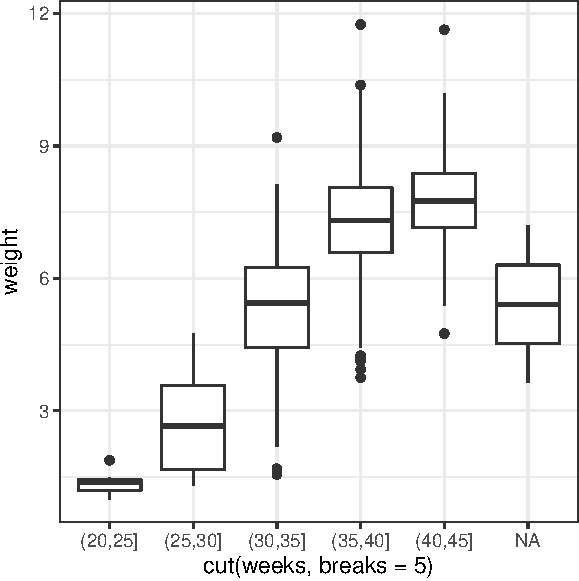
\includegraphics{CorrRegSC_files/figure-latex/unnamed-chunk-4-1} \end{center}

\begin{center}\rule{0.5\linewidth}{0.5pt}\end{center}

\begin{center}\rule{0.5\linewidth}{0.5pt}\end{center}

\hypertarget{creating-scatterplots}{%
\section{Creating scatterplots}\label{creating-scatterplots}}

Creating scatterplots is simple and they are so useful that is it worthwhile to expose yourself to many examples. Over time, you will gain familiarity with the types of patterns that you see. You will begin to recognize how scatterplots can reveal the nature of the relationship between two variables.

In this exercise, and throughout this chapter, we will be using several datasets listed below. These data are available through the \texttt{openintro} package. Briefly:

\begin{itemize}
\item
  The \texttt{mammals} dataset contains information about 39 different species of mammals, including their body weight, brain weight, gestation time, and a few other variables.
\item
  The \texttt{mlbbat10} dataset contains batting statistics for 1,199 Major League Baseball players during the 2010 season.
\item
  The \texttt{bdims} dataset contains body girth and skeletal diameter measurements for 507 physically active individuals.
\item
  The \texttt{smoking} dataset contains information on the smoking habits of 1,691 citizens of the United Kingdom.
\end{itemize}

To see more thorough documentation, use the \texttt{?} or \texttt{help()} functions.

\begin{center}\rule{0.5\linewidth}{0.5pt}\end{center}

\hypertarget{exercise-2}{%
\subsection*{Exercise}\label{exercise-2}}
\addcontentsline{toc}{subsection}{Exercise}

\begin{itemize}
\tightlist
\item
  Using the \texttt{mammals} dataset, create a scatterplot illustrating how the brain weight of a mammal varies as a function of its body weight.
\end{itemize}

\begin{Shaded}
\begin{Highlighting}[]
\KeywordTok{library}\NormalTok{(openintro)}
\CommentTok{# Mammals scatterplot}
\KeywordTok{ggplot}\NormalTok{(}\DataTypeTok{data =}\NormalTok{ mammals, }\KeywordTok{aes}\NormalTok{(}\DataTypeTok{y =}\NormalTok{ brain_wt, }\DataTypeTok{x =}\NormalTok{ body_wt)) }\OperatorTok{+}
\StringTok{  }\KeywordTok{geom_point}\NormalTok{() }\OperatorTok{+}\StringTok{ }
\StringTok{  }\KeywordTok{theme_bw}\NormalTok{() }\OperatorTok{+}\StringTok{ }
\StringTok{  }\KeywordTok{labs}\NormalTok{(}\DataTypeTok{x =} \StringTok{"Body Weight (kg)"}\NormalTok{, }\DataTypeTok{y =} \StringTok{"Brain weight (kg)"}\NormalTok{)}
\end{Highlighting}
\end{Shaded}

\begin{center}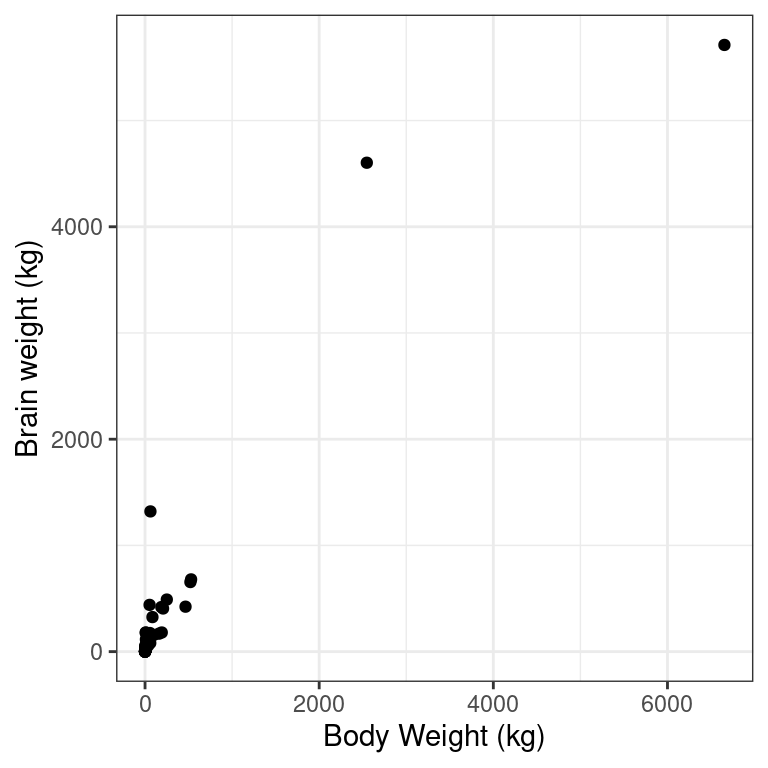
\includegraphics{CorrRegSC_files/figure-latex/unnamed-chunk-5-1} \end{center}

\begin{itemize}
\tightlist
\item
  Using the \texttt{mlbbat10} dataset, create a scatterplot illustrating how the slugging percentage (slg) of a player varies as a function of his on-base percentage (obp).
\end{itemize}

\begin{Shaded}
\begin{Highlighting}[]
\CommentTok{# Baseball player scatterplot}
\NormalTok{p1 <-}\StringTok{ }\KeywordTok{ggplot}\NormalTok{(}\DataTypeTok{data =}\NormalTok{ mlbbat10, }\KeywordTok{aes}\NormalTok{(}\DataTypeTok{y =}\NormalTok{ slg, }\DataTypeTok{x =}\NormalTok{ obp)) }\OperatorTok{+}
\StringTok{  }\KeywordTok{geom_point}\NormalTok{(}\DataTypeTok{alpha =} \FloatTok{0.10}\NormalTok{) }\OperatorTok{+}\StringTok{ }
\StringTok{  }\KeywordTok{theme_bw}\NormalTok{() }\OperatorTok{+}\StringTok{ }
\StringTok{  }\KeywordTok{labs}\NormalTok{(}\DataTypeTok{y =} \StringTok{"Slugging percentage (TB/AB)"}\NormalTok{, }\DataTypeTok{x =} \StringTok{"On base percentage"}\NormalTok{ )}
\NormalTok{p1}
\end{Highlighting}
\end{Shaded}

\begin{center}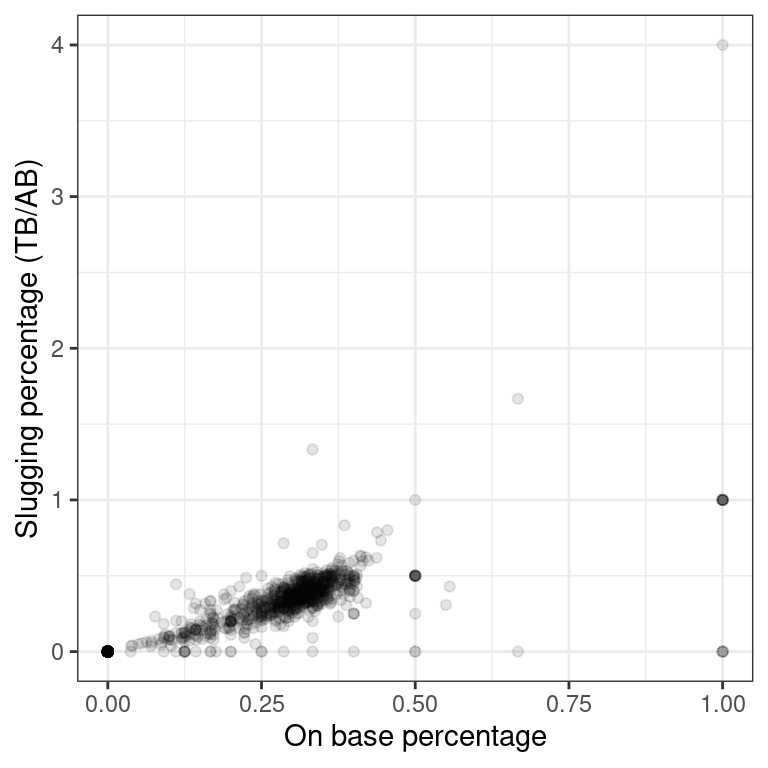
\includegraphics{CorrRegSC_files/figure-latex/unnamed-chunk-6-1} \end{center}

\begin{itemize}
\tightlist
\item
  Using the \texttt{bdims} dataset, create a scatterplot illustrating how a person's weight varies as a function of their height. Use color to separate by sex, which you'll need to coerce to a factor with \texttt{factor()}.
\end{itemize}

\begin{Shaded}
\begin{Highlighting}[]
\CommentTok{# Body dimensions scatterplot}
\NormalTok{p3 <-}\StringTok{ }\KeywordTok{ggplot}\NormalTok{(}\DataTypeTok{data =}\NormalTok{ bdims, }\KeywordTok{aes}\NormalTok{(}\DataTypeTok{y =}\NormalTok{ wgt, }\DataTypeTok{x=}\NormalTok{ hgt, }\DataTypeTok{color =} \KeywordTok{factor}\NormalTok{(sex))) }\OperatorTok{+}\StringTok{ }
\StringTok{  }\KeywordTok{geom_point}\NormalTok{() }\OperatorTok{+}\StringTok{ }
\StringTok{  }\KeywordTok{theme_bw}\NormalTok{() }\OperatorTok{+}\StringTok{ }
\StringTok{  }\KeywordTok{labs}\NormalTok{(}\DataTypeTok{y =} \StringTok{"Weight (kg)"}\NormalTok{, }\DataTypeTok{x =} \StringTok{"Height (cm)"}\NormalTok{)}
\NormalTok{p3}
\end{Highlighting}
\end{Shaded}

\begin{center}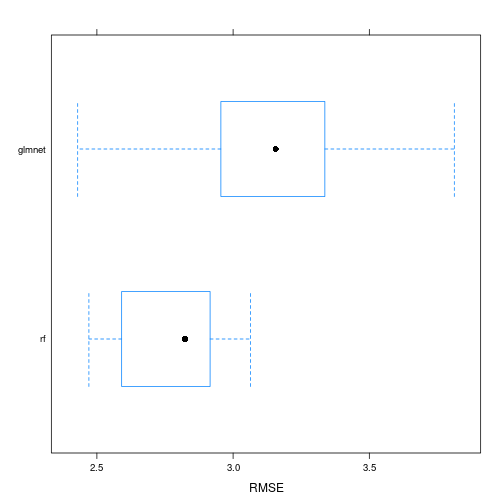
\includegraphics{CorrRegSC_files/figure-latex/unnamed-chunk-7-1} \end{center}

\begin{itemize}
\tightlist
\item
  Using the \texttt{smoking} dataset, create a scatterplot illustrating how the amount that a person smokes on weekdays varies as a function of their age.
\end{itemize}

\begin{Shaded}
\begin{Highlighting}[]
\CommentTok{# Smoking scatterplot}
\KeywordTok{ggplot}\NormalTok{(}\DataTypeTok{data =}\NormalTok{ smoking, }\KeywordTok{aes}\NormalTok{(}\DataTypeTok{y =}\NormalTok{ amt_weekdays, }\DataTypeTok{x =}\NormalTok{ age)) }\OperatorTok{+}\StringTok{ }
\StringTok{  }\KeywordTok{geom_point}\NormalTok{(}\DataTypeTok{alpha =} \FloatTok{0.2}\NormalTok{) }\OperatorTok{+}\StringTok{ }
\StringTok{  }\KeywordTok{theme_bw}\NormalTok{() }\OperatorTok{+}\StringTok{ }
\StringTok{  }\KeywordTok{labs}\NormalTok{(}\DataTypeTok{x =} \StringTok{"Age"}\NormalTok{, }\DataTypeTok{y =} \StringTok{"Number of cigarettes smoked per day on weekdays"}\NormalTok{)}
\end{Highlighting}
\end{Shaded}

\begin{verbatim}
Warning: Removed 1270 rows containing missing values (geom_point).
\end{verbatim}

\begin{center}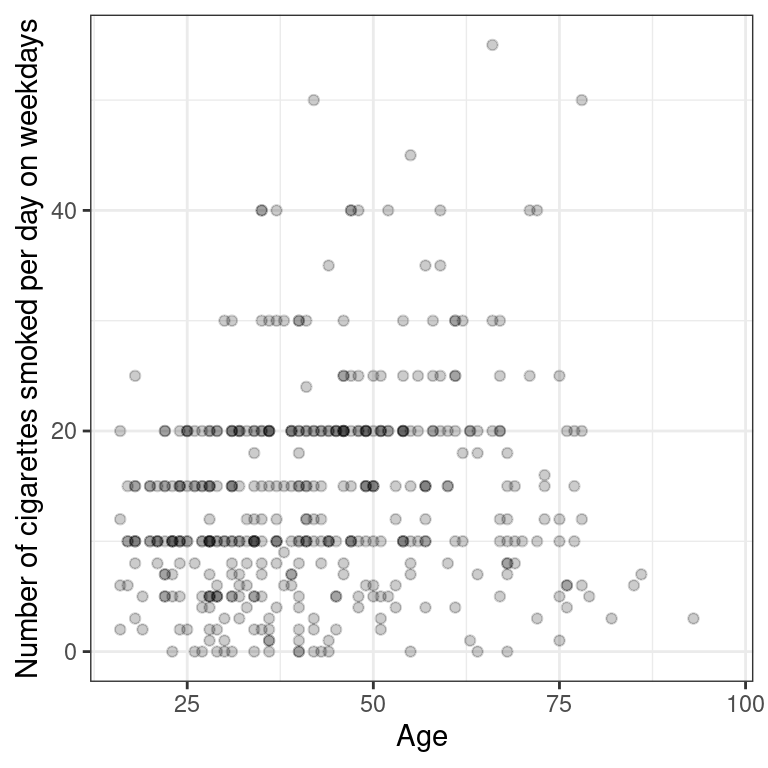
\includegraphics{CorrRegSC_files/figure-latex/unnamed-chunk-8-1} \end{center}

\begin{center}\rule{0.5\linewidth}{0.5pt}\end{center}

\hypertarget{characterizing-scatterplots}{%
\subsection*{Characterizing scatterplots}\label{characterizing-scatterplots}}
\addcontentsline{toc}{subsection}{Characterizing scatterplots}

Figure \ref{fig:sp1} shows the relationship between the poverty rates and high school graduation rates of counties in the United States.

\begin{verbatim}

-- Column specification --------------------------------------------------------
cols(
  .default = col_double()
)
i Use `spec()` for the full column specifications.
\end{verbatim}

\begin{figure}

{\centering 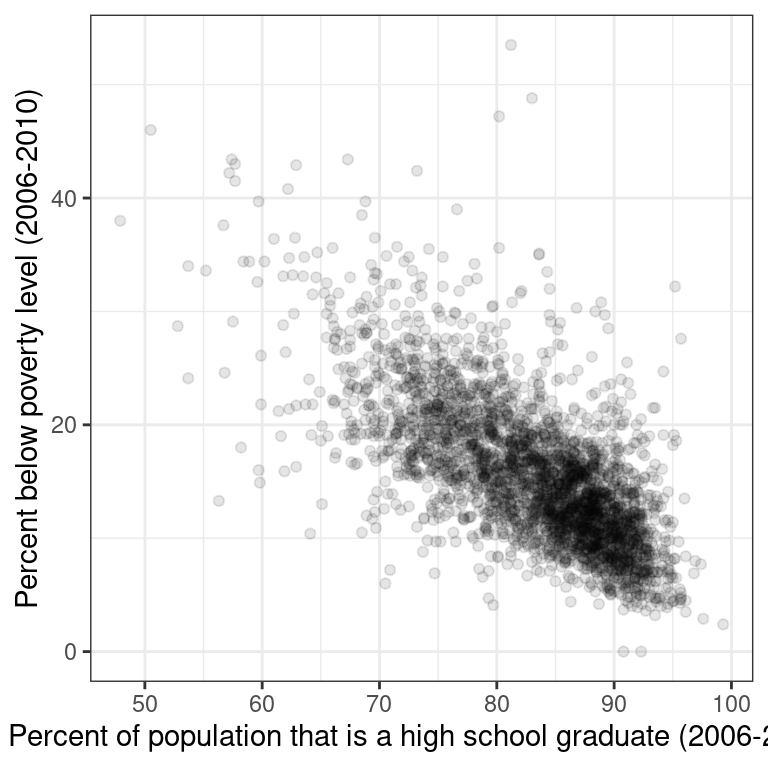
\includegraphics{CorrRegSC_files/figure-latex/sp1-1} 

}

\caption{Poverty versus high school graduation rate}\label{fig:sp1}
\end{figure}

Describe the form, direction, and strength of this relationship.

\begin{itemize}
\item
  Linear, positive, strong
\item
  Linear, negative, weak
\item
  \textbf{Linear, negative, moderately strong}
\item
  Non-linear, negative, strong
\end{itemize}

\begin{center}\rule{0.5\linewidth}{0.5pt}\end{center}

\hypertarget{transformations}{%
\section{Transformations}\label{transformations}}

The relationship between two variables may not be linear. In these cases we can sometimes see strange and even inscrutable patterns in a scatterplot of the data. Sometimes there really is no meaningful relationship between the two variables. Other times, a careful transformation of one or both of the variables can reveal a clear relationship.

Recall the bizarre pattern that you saw in the scatterplot between brain weight and body weight among mammals in a previous exercise. Can we use transformations to clarify this relationship?

\texttt{ggplot2} provides several different mechanisms for viewing transformed relationships. The \texttt{coord\_trans()} function transforms the coordinates of the plot. Alternatively, the \texttt{scale\_x\_log10()} and \texttt{scale\_y\_log10()} functions perform a base-10 log transformation of each axis. Note the differences in the appearance of the axes.

\begin{center}\rule{0.5\linewidth}{0.5pt}\end{center}

\hypertarget{exercise-3}{%
\subsection*{Exercise}\label{exercise-3}}
\addcontentsline{toc}{subsection}{Exercise}

The \texttt{mammals} dataset is available in your workspace.

\begin{itemize}
\tightlist
\item
  Use \texttt{coord\_trans()} to create a scatterplot showing how a mammal's brain weight varies as a function of its body weight, where both the x and y axes are on a \texttt{"log10"} scale.
\end{itemize}

\begin{Shaded}
\begin{Highlighting}[]
\CommentTok{# Scatterplot with coord_trans()}
\KeywordTok{ggplot}\NormalTok{(}\DataTypeTok{data =}\NormalTok{ mammals, }\KeywordTok{aes}\NormalTok{(}\DataTypeTok{y =}\NormalTok{ brain_wt, }\DataTypeTok{x =}\NormalTok{ body_wt)) }\OperatorTok{+}\StringTok{ }
\StringTok{  }\KeywordTok{geom_point}\NormalTok{() }\OperatorTok{+}\StringTok{ }
\StringTok{  }\KeywordTok{coord_trans}\NormalTok{(}\DataTypeTok{x =} \StringTok{"log10"}\NormalTok{, }\DataTypeTok{y =} \StringTok{"log10"}\NormalTok{) }\OperatorTok{+}\StringTok{ }
\StringTok{  }\KeywordTok{theme_bw}\NormalTok{() }\OperatorTok{+}
\StringTok{  }\KeywordTok{labs}\NormalTok{(}\DataTypeTok{x =} \StringTok{"Total body weight of the mammal (in kg)"}\NormalTok{,}
       \DataTypeTok{y =} \StringTok{"Brain weight of the mammal (in kg)"}\NormalTok{)}
\end{Highlighting}
\end{Shaded}

\begin{center}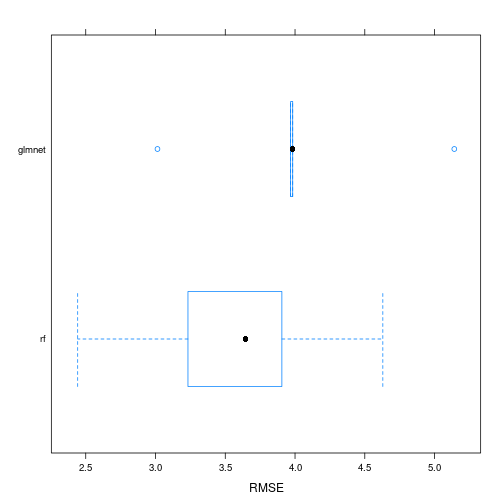
\includegraphics{CorrRegSC_files/figure-latex/unnamed-chunk-9-1} \end{center}

\begin{itemize}
\tightlist
\item
  Use \texttt{scale\_x\_log10()} and \texttt{scale\_y\_log10()} to achieve the same effect but with different axis labels and grid lines.
\end{itemize}

\begin{Shaded}
\begin{Highlighting}[]
\CommentTok{# Scatterplot with scale_x_log10() and scale_y_log10()}
\NormalTok{p4 <-}\StringTok{ }\KeywordTok{ggplot}\NormalTok{(}\DataTypeTok{data =}\NormalTok{ mammals, }\KeywordTok{aes}\NormalTok{(}\DataTypeTok{x =}\NormalTok{ body_wt, }\DataTypeTok{y =}\NormalTok{ brain_wt)) }\OperatorTok{+}
\StringTok{  }\KeywordTok{geom_point}\NormalTok{() }\OperatorTok{+}
\StringTok{  }\KeywordTok{scale_x_log10}\NormalTok{() }\OperatorTok{+}\StringTok{ }
\StringTok{  }\KeywordTok{scale_y_log10}\NormalTok{() }\OperatorTok{+}\StringTok{ }
\StringTok{  }\KeywordTok{theme_bw}\NormalTok{() }\OperatorTok{+}\StringTok{ }
\StringTok{  }\KeywordTok{labs}\NormalTok{(}\DataTypeTok{x =} \StringTok{"Total body weight of the mammal (in kg)"}\NormalTok{,}
       \DataTypeTok{y =} \StringTok{"Brain weight of the mammal (in kg)"}\NormalTok{)}
\NormalTok{p4}
\end{Highlighting}
\end{Shaded}

\begin{center}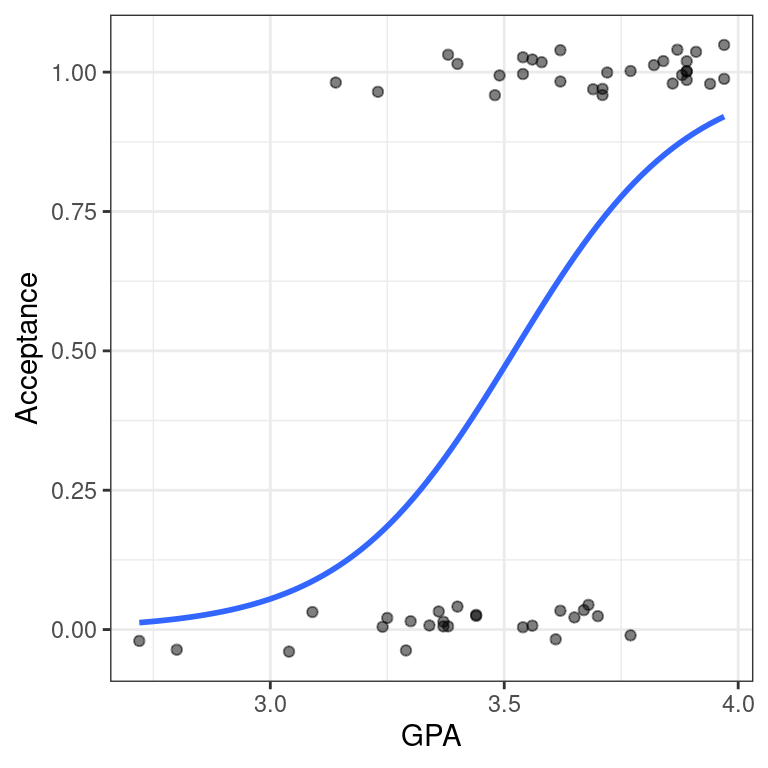
\includegraphics{CorrRegSC_files/figure-latex/unnamed-chunk-10-1} \end{center}

\hypertarget{identifying-outliers}{%
\section{Identifying outliers}\label{identifying-outliers}}

In Chapter \ref{modelfit}, we will discuss how outliers can affect the results of a linear regression model and how we can deal with them. For now, it is enough to simply identify them and note how the relationship between two variables may change as a result of removing outliers.

Recall that in the baseball example earlier in the chapter, most of the points were clustered in the lower left corner of the plot, making it difficult to see the general pattern of the majority of the data. This difficulty was caused by a few outlying players whose on-base percentages (OBPs) were exceptionally high. These values are present in our dataset only because these players had very few batting opportunities.

Both OBP and SLG are known as rate statistics, since they measure the frequency of certain events (as opposed to their count). In order to compare these rates sensibly, it makes sense to include only players with a reasonable number of opportunities, so that these observed rates have the chance to approach their long-run frequencies.

In Major League Baseball, batters qualify for the batting title only if they have 3.1 plate appearances per game. This translates into roughly 502 plate appearances in a 162-game season. The \texttt{mlbbat10} dataset does not include plate appearances as a variable, but we can use at-bats (\texttt{at\_bat}) -- which constitute a subset of plate appearances -- as a proxy.

\begin{center}\rule{0.5\linewidth}{0.5pt}\end{center}

\hypertarget{exercise-4}{%
\subsection*{Exercise}\label{exercise-4}}
\addcontentsline{toc}{subsection}{Exercise}

\begin{itemize}
\tightlist
\item
  Use \texttt{filter()} to create a scatterplot for \texttt{slg} as a function of \texttt{obp} among players who had at least 200 at-bats.
\end{itemize}

\begin{Shaded}
\begin{Highlighting}[]
\KeywordTok{library}\NormalTok{(dplyr)}
\CommentTok{# Scatterplot of slg vs. obp}
\NormalTok{ntib <-}\StringTok{ }\NormalTok{mlbbat10 }\OperatorTok\StringTok{ }
\StringTok{  }\KeywordTok{filter}\NormalTok{(at_bat }\OperatorTok{>=}\StringTok{ }\DecValTok{200}\NormalTok{)}
\NormalTok{p2 <-}\StringTok{ }\KeywordTok{ggplot}\NormalTok{(}\DataTypeTok{data =}\NormalTok{ ntib, }\KeywordTok{aes}\NormalTok{(}\DataTypeTok{y =}\NormalTok{ slg, }\DataTypeTok{x =}\NormalTok{ obp)) }\OperatorTok{+}\StringTok{ }
\StringTok{  }\KeywordTok{geom_point}\NormalTok{() }\OperatorTok{+}
\StringTok{  }\KeywordTok{theme_bw}\NormalTok{()}
\NormalTok{p2}
\end{Highlighting}
\end{Shaded}

\begin{center}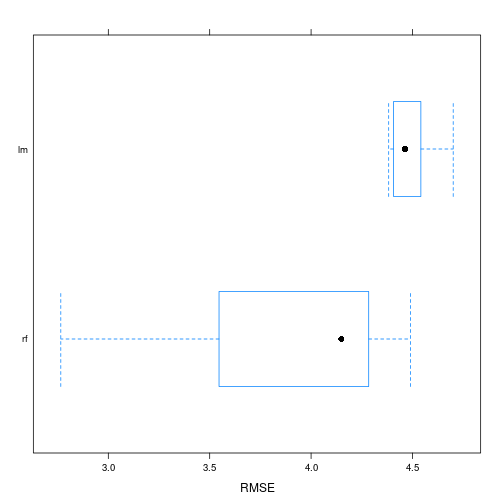
\includegraphics{CorrRegSC_files/figure-latex/unnamed-chunk-11-1} \end{center}

\begin{itemize}
\tightlist
\item
  Find the row of \texttt{mlbbat10} corresponding to the one player with at least 200 at-bats whose \texttt{obp} was below 0.200.
\end{itemize}

\begin{Shaded}
\begin{Highlighting}[]
\CommentTok{# Identify the outlying player}
\NormalTok{mlbbat10 }\OperatorTok\StringTok{ }
\StringTok{  }\KeywordTok{filter}\NormalTok{(at_bat }\OperatorTok{>=}\DecValTok{200}\NormalTok{, obp }\OperatorTok{<}\StringTok{ }\FloatTok{0.2}\NormalTok{)}
\end{Highlighting}
\end{Shaded}

\begin{verbatim}
# A tibble: 1 x 19
  name  team  position  game at_bat   run   hit double triple home_run   rbi
  <fct> <fct> <fct>    <dbl>  <dbl> <dbl> <dbl>  <dbl>  <dbl>    <dbl> <dbl>
1 B Wo~ LAA   3B          81    226    20    33      2      0        4    14
# ... with 8 more variables: total_base <dbl>, walk <dbl>, strike_out <dbl>,
#   stolen_base <dbl>, caught_stealing <dbl>, obp <dbl>, slg <dbl>,
#   bat_avg <dbl>
\end{verbatim}

\hypertarget{correlation}{%
\chapter{Correlation}\label{correlation}}

This chapter introduces correlation as a means of quantifying bivariate relationships.

\hypertarget{understanding-correlation-scale}{%
\subsection*{Understanding correlation scale}\label{understanding-correlation-scale}}
\addcontentsline{toc}{subsection}{Understanding correlation scale}

In a scientific paper, three correlations are reported with the following values:

\begin{enumerate}
\def\labelenumi{\arabic{enumi}.}
\tightlist
\item
  -0.395
\item
  1.827
\item
  0.738
\end{enumerate}

Choose the correct interpretation of these findings.

\begin{enumerate}
\def\labelenumi{\arabic{enumi}.}
\tightlist
\item
  is invalid.
\item
  \textbf{is invalid.}
\item
  is invalid.
\end{enumerate}

\begin{center}\rule{0.5\linewidth}{0.5pt}\end{center}

\hypertarget{understanding-correlation-sign}{%
\subsection*{Understanding correlation sign}\label{understanding-correlation-sign}}
\addcontentsline{toc}{subsection}{Understanding correlation sign}

In a scientific paper, three correlations are reported with the following values:

\begin{enumerate}
\def\labelenumi{\arabic{enumi}.}
\tightlist
\item
  0.582
\item
  0.134
\item
  -0.795
\end{enumerate}

Which of these values represents the strongest correlation?

Possible Answers

\begin{itemize}
\item
  0.582
\item
  0.134
\item
  \textbf{-0.795}
\item
  Can't tell!
\end{itemize}

\begin{center}\rule{0.5\linewidth}{0.5pt}\end{center}

\hypertarget{computing-correlation}{%
\section{Computing correlation}\label{computing-correlation}}

The \texttt{cor(x,\ y)} function will compute the Pearson product-moment correlation between variables, \texttt{x} and \texttt{y}. Since this quantity is symmetric with respect to \texttt{x} and \texttt{y}, it doesn't matter in which order you put the variables.

At the same time, the \texttt{cor()} function is very conservative when it encounters missing data (e.g.~\texttt{NA}s). The \texttt{use} argument allows you to override the default behavior of returning \texttt{NA} whenever any of the values encountered is \texttt{NA}. Setting the \texttt{use} argument to \texttt{"pairwise.complete.obs"} allows \texttt{cor()} to compute the correlation coefficient for those observations where the values of \texttt{x} and \texttt{y} are both not missing.

\begin{center}\rule{0.5\linewidth}{0.5pt}\end{center}

\hypertarget{exercise-5}{%
\subsection*{Exercise}\label{exercise-5}}
\addcontentsline{toc}{subsection}{Exercise}

\begin{itemize}
\tightlist
\item
  Use \texttt{cor()} to compute the correlation between the birthweight of babies in the \texttt{ncbirths} dataset and their mother's age. There is no missing data in either variable.
\end{itemize}

\begin{Shaded}
\begin{Highlighting}[]
\KeywordTok{library}\NormalTok{(openintro)}
\NormalTok{DT}\OperatorTok{::}\KeywordTok{datatable}\NormalTok{(ncbirths)}
\end{Highlighting}
\end{Shaded}

\begin{Shaded}
\begin{Highlighting}[]
\CommentTok{# Compute correlation}
\NormalTok{ncbirths }\OperatorTok
\StringTok{  }\KeywordTok{summarize}\NormalTok{(}\DataTypeTok{N =} \KeywordTok{n}\NormalTok{(), }\DataTypeTok{r =} \KeywordTok{cor}\NormalTok{(weight, mage))}
\end{Highlighting}
\end{Shaded}

\begin{verbatim}
# A tibble: 1 x 2
      N      r
  <int>  <dbl>
1  1000 0.0551
\end{verbatim}

\begin{itemize}
\tightlist
\item
  Compute the correlation between the birthweight and the number of weeks of gestation for all non-missing pairs.
\end{itemize}

\begin{Shaded}
\begin{Highlighting}[]
\CommentTok{# Compute correlation for all non-missing pairs}
\NormalTok{ncbirths }\OperatorTok
\StringTok{  }\KeywordTok{summarize}\NormalTok{(}\DataTypeTok{N =} \KeywordTok{n}\NormalTok{(), }\DataTypeTok{r =} \KeywordTok{cor}\NormalTok{(weight, weeks, }
                             \DataTypeTok{use =} \StringTok{"pairwise.complete.obs"}\NormalTok{))}
\end{Highlighting}
\end{Shaded}

\begin{verbatim}
# A tibble: 1 x 2
      N     r
  <int> <dbl>
1  1000 0.670
\end{verbatim}

\begin{center}\rule{0.5\linewidth}{0.5pt}\end{center}

\hypertarget{exploring-anscombe}{%
\section{Exploring Anscombe}\label{exploring-anscombe}}

In 1973, Francis Anscombe famously created four datasets with remarkably similar numerical properties, but obviously different graphic relationships. The \texttt{Anscombe} dataset contains the \texttt{x} and \texttt{y} coordinates for these four datasets, along with a grouping variable, \texttt{set}, that distinguishes the quartet.

It may be helpful to remind yourself of the graphic relationship by viewing the four scatterplots:

\begin{Shaded}
\begin{Highlighting}[]
\NormalTok{dat <-}\StringTok{ }\NormalTok{datasets}\OperatorTok{::}\NormalTok{anscombe}
\NormalTok{Anscombe <-}\StringTok{ }\KeywordTok{data.frame}\NormalTok{(}
    \DataTypeTok{set  =} \KeywordTok{rep}\NormalTok{(}\DecValTok{1}\OperatorTok{:}\DecValTok{4}\NormalTok{, }\DataTypeTok{each =} \DecValTok{11}\NormalTok{),}
    \DataTypeTok{x =} \KeywordTok{unlist}\NormalTok{(dat[ ,}\KeywordTok{c}\NormalTok{(}\DecValTok{1}\OperatorTok{:}\DecValTok{4}\NormalTok{)]),}
    \DataTypeTok{y =} \KeywordTok{unlist}\NormalTok{(dat[ ,}\KeywordTok{c}\NormalTok{(}\DecValTok{5}\OperatorTok{:}\DecValTok{8}\NormalTok{)])}
\NormalTok{    )}
\KeywordTok{rownames}\NormalTok{(Anscombe) <-}\StringTok{ }\OtherTok{NULL}
\KeywordTok{head}\NormalTok{(Anscombe)}
\end{Highlighting}
\end{Shaded}

\begin{verbatim}
  set  x    y
1   1 10 8.04
2   1  8 6.95
3   1 13 7.58
4   1  9 8.81
5   1 11 8.33
6   1 14 9.96
\end{verbatim}

\begin{Shaded}
\begin{Highlighting}[]
\CommentTok{#}
\KeywordTok{ggplot}\NormalTok{(}\DataTypeTok{data =}\NormalTok{ Anscombe, }\KeywordTok{aes}\NormalTok{(}\DataTypeTok{x =}\NormalTok{ x, }\DataTypeTok{y =}\NormalTok{ y)) }\OperatorTok{+}
\StringTok{  }\KeywordTok{geom_point}\NormalTok{() }\OperatorTok{+}
\StringTok{  }\KeywordTok{facet_wrap}\NormalTok{(}\KeywordTok{vars}\NormalTok{(set)) }\OperatorTok{+}\StringTok{ }
\StringTok{  }\KeywordTok{theme_bw}\NormalTok{()}
\end{Highlighting}
\end{Shaded}

\begin{center}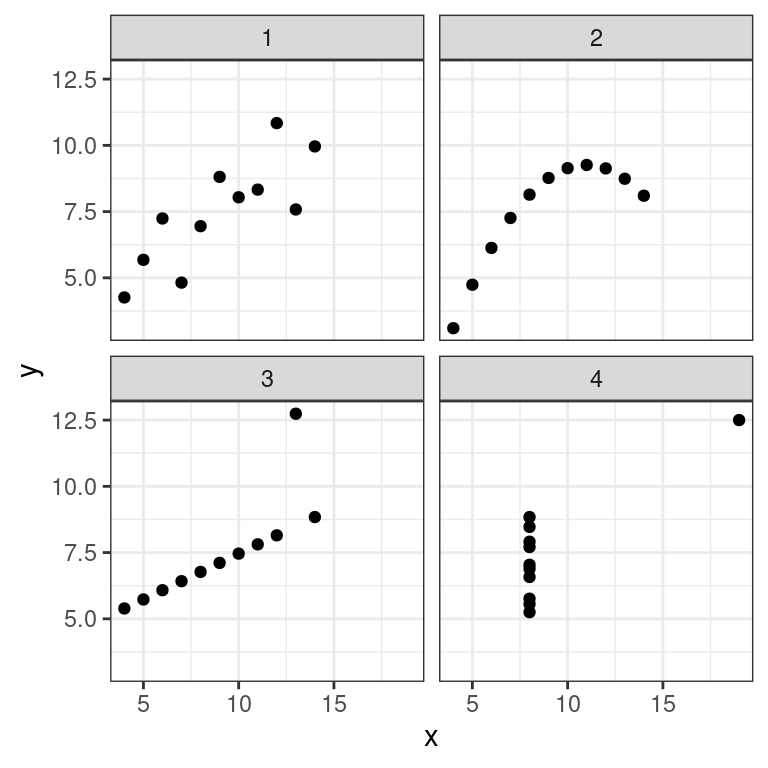
\includegraphics{CorrRegSC_files/figure-latex/unnamed-chunk-15-1} \end{center}

\begin{center}\rule{0.5\linewidth}{0.5pt}\end{center}

\hypertarget{exercise-6}{%
\subsection*{Exercise}\label{exercise-6}}
\addcontentsline{toc}{subsection}{Exercise}

For each of the four sets of data points in the \texttt{Anscombe} dataset, compute the following in the order specified. Don't worry about naming any of the variables other than the first in your call to \texttt{summarize()}.

\begin{itemize}
\item
  Number of observations, \texttt{N}
\item
  Mean of \texttt{x}
\item
  Standard deviation of \texttt{x}
\item
  Mean of \texttt{y}
\item
  Standard deviation of \texttt{y}
\item
  Correlation coefficient between \texttt{x} and \texttt{y}
\end{itemize}

\begin{Shaded}
\begin{Highlighting}[]
\CommentTok{# Compute properties of Anscombe}
\NormalTok{Anscombe }\OperatorTok
\StringTok{  }\KeywordTok{group_by}\NormalTok{(set) }\OperatorTok
\StringTok{  }\KeywordTok{summarize}\NormalTok{(}\DataTypeTok{N =} \KeywordTok{n}\NormalTok{(), }\KeywordTok{mean}\NormalTok{(x), }\KeywordTok{sd}\NormalTok{(x), }\KeywordTok{mean}\NormalTok{(y), }\KeywordTok{sd}\NormalTok{(y), }\KeywordTok{cor}\NormalTok{(x, y))}
\end{Highlighting}
\end{Shaded}

\begin{verbatim}
# A tibble: 4 x 7
    set     N `mean(x)` `sd(x)` `mean(y)` `sd(y)` `cor(x, y)`
* <int> <int>     <dbl>   <dbl>     <dbl>   <dbl>       <dbl>
1     1    11         9    3.32      7.50    2.03       0.816
2     2    11         9    3.32      7.50    2.03       0.816
3     3    11         9    3.32      7.5     2.03       0.816
4     4    11         9    3.32      7.50    2.03       0.817
\end{verbatim}

\begin{center}\rule{0.5\linewidth}{0.5pt}\end{center}

\hypertarget{perception-of-correlation}{%
\subsection*{Perception of correlation}\label{perception-of-correlation}}
\addcontentsline{toc}{subsection}{Perception of correlation}

Recall Figure \ref{fig:sp1} which displays the poverty rate of counties in the United States and the high school graduation rate in those counties from the previous chapter. Which of the following values is the correct correlation between poverty rate and high school graduation rate?

\begin{itemize}
\tightlist
\item
  -0.861
\item
  \textbf{-0.681}
\item
  -0.186
\item
  0.186
\item
  0.681
\item
  0.861
\end{itemize}

\begin{Shaded}
\begin{Highlighting}[]
\KeywordTok{library}\NormalTok{(openintro)}
\NormalTok{cc }\OperatorTok\StringTok{ }
\StringTok{  }\KeywordTok{summarize}\NormalTok{(}\DataTypeTok{r =} \KeywordTok{cor}\NormalTok{(poverty, hs_grad)) }\OperatorTok\StringTok{ }
\StringTok{  }\KeywordTok{round}\NormalTok{(}\DecValTok{3}\NormalTok{)}
\end{Highlighting}
\end{Shaded}

\begin{verbatim}
# A tibble: 1 x 1
       r
   <dbl>
1 -0.685
\end{verbatim}

\begin{center}\rule{0.5\linewidth}{0.5pt}\end{center}

\hypertarget{perception-of-correlation-2}{%
\subsection*{Perception of correlation (2)}\label{perception-of-correlation-2}}
\addcontentsline{toc}{subsection}{Perception of correlation (2)}

Estimating the value of the correlation coefficient between two quantities from their scatterplot can be tricky. \href{https://statistics.stanford.edu/sites/g/files/sbiybj6031/f/EFS\%20NSF\%20206.pdf}{Statisticians have shown that} people's perception of the strength of these relationships can be influenced by design choices like the x and y scales.

Nevertheless, with some practice your perception of correlation will improve. Study the four scatterplots in Figure \ref{fig:fourplots}, each of which you've seen in a previous exercise.

\begin{Shaded}
\begin{Highlighting}[]
\KeywordTok{library}\NormalTok{(gridExtra)}
\KeywordTok{grid.arrange}\NormalTok{(p1, p2, p3, p4)}
\end{Highlighting}
\end{Shaded}

\begin{figure}

{\centering 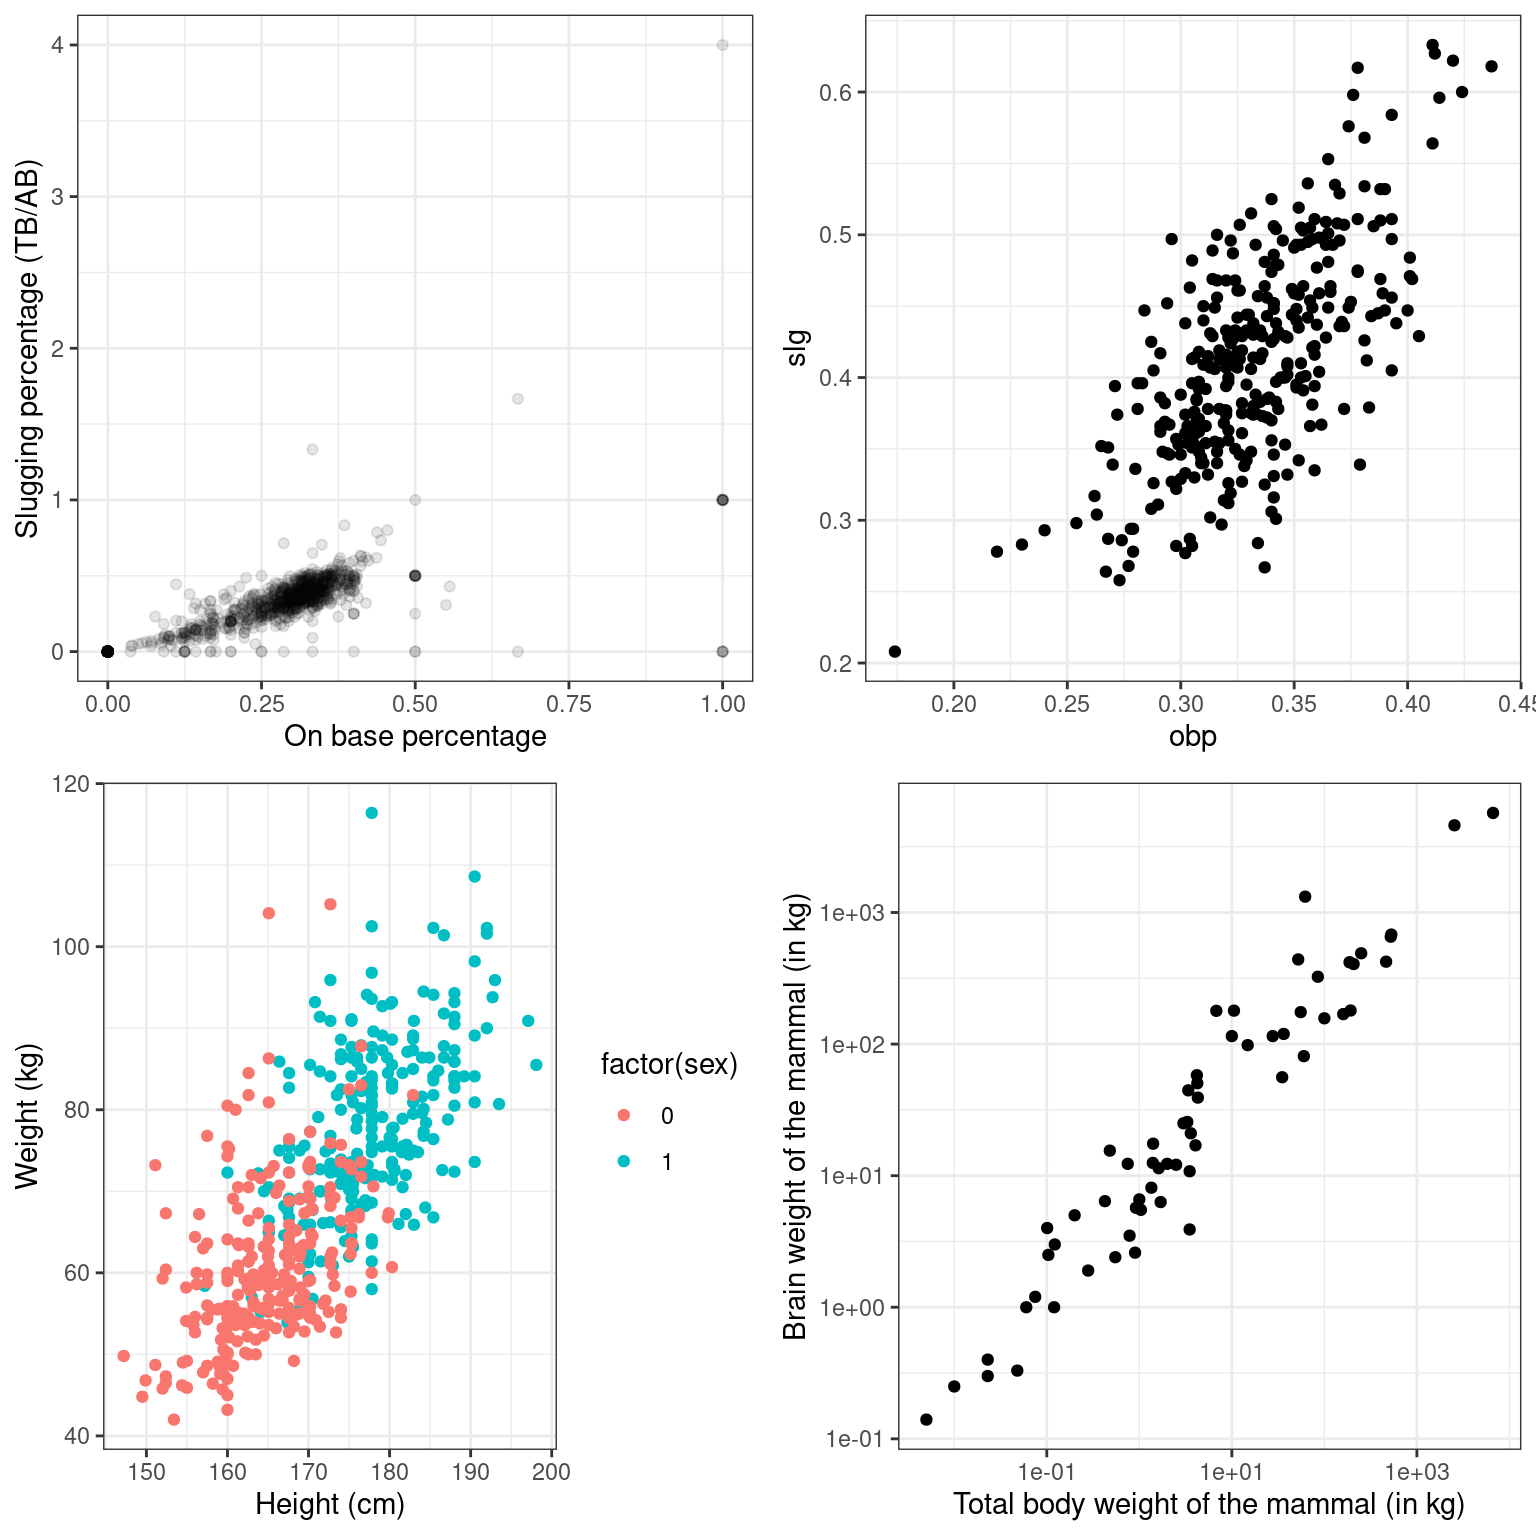
\includegraphics{CorrRegSC_files/figure-latex/fourplots-1} 

}

\caption{Four scatterplots}\label{fig:fourplots}
\end{figure}

Jot down your best estimate of the value of the correlation coefficient between each pair of variables. Then, compare these values to the actual values you compute in this exercise.

\begin{center}\rule{0.5\linewidth}{0.5pt}\end{center}

\hypertarget{exercise-7}{%
\subsection*{Exercise}\label{exercise-7}}
\addcontentsline{toc}{subsection}{Exercise}

Each graph in the plotting window corresponds to an instruction below. Compute the correlation between\ldots{}

\begin{itemize}
\tightlist
\item
  \texttt{obp} and \texttt{slg} for all players in the \texttt{mlbbat10} dataset.
\end{itemize}

\begin{Shaded}
\begin{Highlighting}[]
\CommentTok{# Correlation for all baseball players}
\NormalTok{mlbbat10 }\OperatorTok\StringTok{ }
\StringTok{  }\KeywordTok{summarize}\NormalTok{(}\DataTypeTok{r =} \KeywordTok{cor}\NormalTok{(obp, slg))}
\end{Highlighting}
\end{Shaded}

\begin{verbatim}
# A tibble: 1 x 1
      r
  <dbl>
1 0.815
\end{verbatim}

\begin{itemize}
\tightlist
\item
  \texttt{obp} and \texttt{slg} for all players in the \texttt{mlbbat10} dataset with at least 200 at-bats.
\end{itemize}

\begin{Shaded}
\begin{Highlighting}[]
\CommentTok{# Correlation for all players with at least 200 ABs}
\NormalTok{mlbbat10 }\OperatorTok\StringTok{ }
\StringTok{  }\KeywordTok{filter}\NormalTok{(at_bat }\OperatorTok{>=}\StringTok{ }\DecValTok{200}\NormalTok{) }\OperatorTok\StringTok{ }
\StringTok{  }\KeywordTok{summarize}\NormalTok{(}\DataTypeTok{r =} \KeywordTok{cor}\NormalTok{(obp, slg))}
\end{Highlighting}
\end{Shaded}

\begin{verbatim}
# A tibble: 1 x 1
      r
  <dbl>
1 0.686
\end{verbatim}

\begin{itemize}
\tightlist
\item
  Height and weight for each sex in the \texttt{bdims} dataset.
\end{itemize}

\begin{Shaded}
\begin{Highlighting}[]
\CommentTok{# Correlation of body dimensions}
\NormalTok{bdims }\OperatorTok
\StringTok{  }\KeywordTok{group_by}\NormalTok{(sex) }\OperatorTok
\StringTok{  }\KeywordTok{summarize}\NormalTok{(}\DataTypeTok{N =} \KeywordTok{n}\NormalTok{(), }\DataTypeTok{r =} \KeywordTok{cor}\NormalTok{(hgt, wgt))}
\end{Highlighting}
\end{Shaded}

\begin{verbatim}
# A tibble: 2 x 3
    sex     N     r
* <int> <int> <dbl>
1     0   260 0.431
2     1   247 0.535
\end{verbatim}

\begin{itemize}
\tightlist
\item
  Body weight and brain weight for all species of mammals. Alongside this computation, compute the correlation between the same two quantities after taking their natural logarithms.
\end{itemize}

\begin{Shaded}
\begin{Highlighting}[]
\CommentTok{# Correlation among mammals, with and without log}
\NormalTok{mammals }\OperatorTok
\StringTok{  }\KeywordTok{summarize}\NormalTok{(}\DataTypeTok{N =} \KeywordTok{n}\NormalTok{(), }
            \DataTypeTok{r =} \KeywordTok{cor}\NormalTok{(brain_wt, body_wt), }
            \DataTypeTok{r_log =} \KeywordTok{cor}\NormalTok{(}\KeywordTok{log}\NormalTok{(brain_wt), }\KeywordTok{log}\NormalTok{(body_wt)))}
\end{Highlighting}
\end{Shaded}

\begin{verbatim}
# A tibble: 1 x 3
      N     r r_log
  <int> <dbl> <dbl>
1    62 0.934 0.960
\end{verbatim}

\begin{center}\rule{0.5\linewidth}{0.5pt}\end{center}

\hypertarget{interpreting-correlation-in-context}{%
\subsection*{Interpreting correlation in context}\label{interpreting-correlation-in-context}}
\addcontentsline{toc}{subsection}{Interpreting correlation in context}

Recall Figure \ref{fig:sp1} where you previously determined the value of the correlation coefficient between the poverty rate of counties in the United States and the high school graduation rate in those counties was -0.681. Choose the correct interpretation of this value.

\begin{itemize}
\item
  People who graduate from high school are less likely to be poor.
\item
  Counties with lower high school graduation rates are likely to have lower poverty rates.
\item
  \textbf{Counties with lower high school graduation rates are likely to have higher poverty rates.}
\item
  Because the correlation is negative, there is no relationship between poverty rates and high school graduate rates.
\item
  Having a higher percentage of high school graduates in a county results in that county having lower poverty rates.
\end{itemize}

\begin{center}\rule{0.5\linewidth}{0.5pt}\end{center}

\hypertarget{correlation-and-causation}{%
\subsection*{Correlation and causation}\label{correlation-and-causation}}
\addcontentsline{toc}{subsection}{Correlation and causation}

In the San Francisco Bay Area from 1960-1967, the correlation between the birthweight of 1,236 babies and the length of their gestational period was 0.408. Which of the following conclusions is \textbf{not} a valid statistical interpretation of these results.

\begin{itemize}
\item
  We observed that babies with longer gestational periods tended to be heavier at birth.
\item
  It may be that a longer gestational period contributes to a heavier birthweight among babies, but a randomized, controlled experiment is needed to confirm this observation.
\item
  \textbf{Staying in the womb longer causes babies to be heavier when they are born.}
\item
  These data suggest that babies with longer gestational periods tend to be heavier at birth, but there are many potential confounding factors that were not taken into account.
\end{itemize}

\begin{center}\rule{0.5\linewidth}{0.5pt}\end{center}

\hypertarget{spurious-correlation-in-random-data}{%
\section{Spurious correlation in random data}\label{spurious-correlation-in-random-data}}

Statisticians must always be skeptical of potentially spurious correlations. Human beings are very good at seeing patterns in data, sometimes when the patterns themselves are actually just random noise. To illustrate how easy it can be to fall into this trap, we will look for patterns in truly random data.

The noise dataset contains 20 sets of \texttt{x} and \texttt{y} variables drawn at random from a standard normal distribution. Each set, denoted as \texttt{z}, has 50 observations of \texttt{x}, \texttt{y} pairs. Do you see any pairs of variables that might be meaningfully correlated? Are all of the correlation coefficients close to zero?

\begin{Shaded}
\begin{Highlighting}[]
\CommentTok{# Create noise}
\KeywordTok{set.seed}\NormalTok{(}\DecValTok{9}\NormalTok{)}
\NormalTok{noise <-}\StringTok{ }\KeywordTok{data.frame}\NormalTok{(}\DataTypeTok{x =} \KeywordTok{rnorm}\NormalTok{(}\DecValTok{1000}\NormalTok{), }\DataTypeTok{y =} \KeywordTok{rnorm}\NormalTok{(}\DecValTok{1000}\NormalTok{), }\DataTypeTok{z =} \KeywordTok{rep}\NormalTok{(}\DecValTok{1}\OperatorTok{:}\DecValTok{20}\NormalTok{, }\DecValTok{50}\NormalTok{))}
\end{Highlighting}
\end{Shaded}

\begin{itemize}
\tightlist
\item
  Create a faceted scatterplot that shows the relationship between each of the 20 sets of pairs of random variables \texttt{x} and \texttt{y}. You will need the \texttt{facet\_wrap()} function for this.
\end{itemize}

\begin{Shaded}
\begin{Highlighting}[]
\CommentTok{# Create faceted scatterplot}
\KeywordTok{ggplot}\NormalTok{(}\DataTypeTok{dat =}\NormalTok{ noise, }\KeywordTok{aes}\NormalTok{(}\DataTypeTok{x=}\NormalTok{ x, }\DataTypeTok{y =}\NormalTok{ y)) }\OperatorTok{+}\StringTok{ }
\StringTok{  }\KeywordTok{geom_point}\NormalTok{() }\OperatorTok{+}\StringTok{ }
\StringTok{  }\KeywordTok{facet_wrap}\NormalTok{(}\KeywordTok{vars}\NormalTok{(z)) }\OperatorTok{+}\StringTok{ }
\StringTok{  }\KeywordTok{theme_bw}\NormalTok{()}
\end{Highlighting}
\end{Shaded}

\begin{center}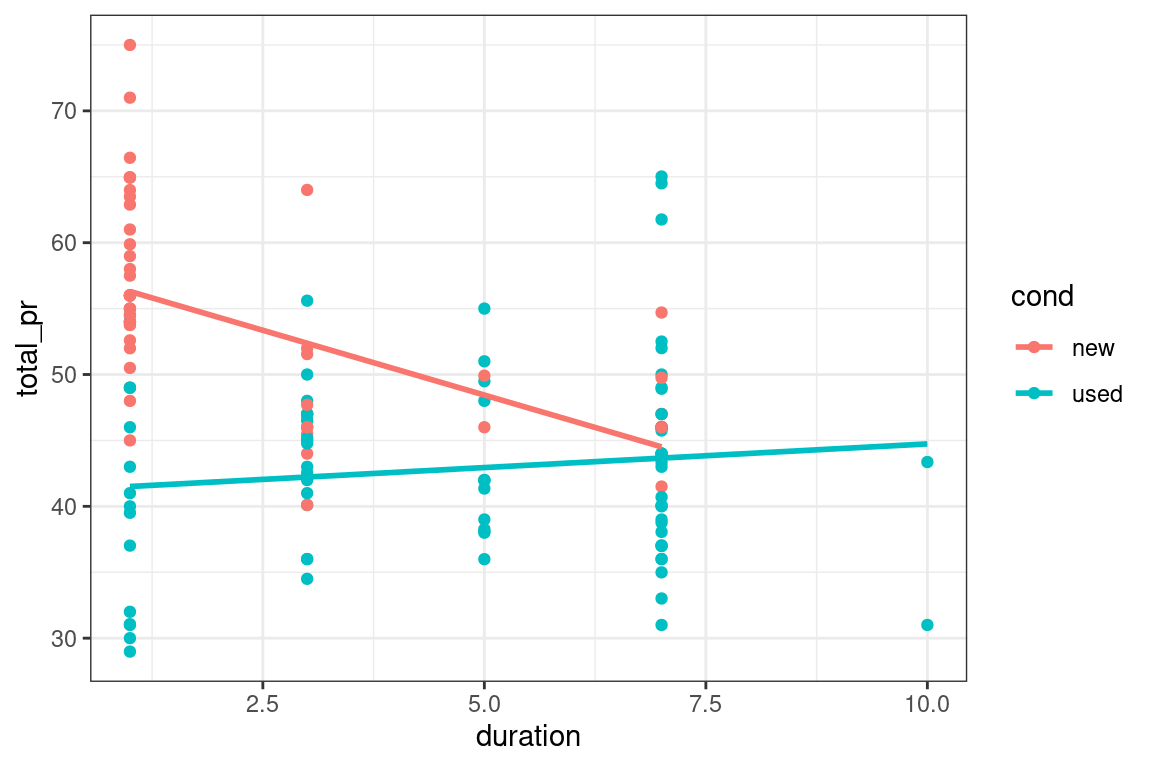
\includegraphics{CorrRegSC_files/figure-latex/unnamed-chunk-23-1} \end{center}

\begin{itemize}
\tightlist
\item
  Compute the actual correlation between each of the 20 sets of pairs of \texttt{x} and \texttt{y}.
\end{itemize}

\begin{Shaded}
\begin{Highlighting}[]
\CommentTok{# Compute correlations for each dataset}
\NormalTok{noise_summary <-}\StringTok{ }\NormalTok{noise }\OperatorTok
\StringTok{  }\KeywordTok{group_by}\NormalTok{(z) }\OperatorTok
\StringTok{  }\KeywordTok{summarize}\NormalTok{(}\DataTypeTok{N =} \KeywordTok{n}\NormalTok{(), }\DataTypeTok{spurious_cor =} \KeywordTok{cor}\NormalTok{(x, y))}
\NormalTok{noise_summary}
\end{Highlighting}
\end{Shaded}

\begin{verbatim}
# A tibble: 20 x 3
       z     N spurious_cor
 * <int> <int>        <dbl>
 1     1    50    -0.104   
 2     2    50    -0.0704  
 3     3    50     0.0185  
 4     4    50    -0.161   
 5     5    50    -0.131   
 6     6    50    -0.0356  
 7     7    50    -0.00713 
 8     8    50    -0.141   
 9     9    50    -0.0564  
10    10    50     0.216   
11    11    50    -0.246   
12    12    50    -0.175   
13    13    50    -0.223   
14    14    50     0.0175  
15    15    50    -0.000720
16    16    50     0.149   
17    17    50    -0.0179  
18    18    50     0.0839  
19    19    50    -0.221   
20    20    50    -0.0969  
\end{verbatim}

\begin{itemize}
\tightlist
\item
  Identify the datasets that show non-trivial correlation of greater than 0.2 in absolute value.
\end{itemize}

\begin{Shaded}
\begin{Highlighting}[]
\CommentTok{# Isolate sets with correlations above 0.2 in absolute strength}
\NormalTok{noise_summary }\OperatorTok\StringTok{ }
\StringTok{  }\KeywordTok{filter}\NormalTok{(}\KeywordTok{abs}\NormalTok{(spurious_cor) }\OperatorTok{>=}\StringTok{ }\FloatTok{0.2}\NormalTok{)}
\end{Highlighting}
\end{Shaded}

\begin{verbatim}
# A tibble: 4 x 3
      z     N spurious_cor
  <int> <int>        <dbl>
1    10    50        0.216
2    11    50       -0.246
3    13    50       -0.223
4    19    50       -0.221
\end{verbatim}

\hypertarget{simple-linear-regression}{%
\chapter{Simple linear regression}\label{simple-linear-regression}}

With the notion of correlation under your belt, we'll now turn our attention to simple linear models in this chapter.

\hypertarget{the-best-fit-line}{%
\section{The ``best fit'' line}\label{the-best-fit-line}}

The simple linear regression model for a numeric response as a function of a numeric explanatory variable can be visualized on the corresponding scatterplot by a straight line. This is a ``best fit'' line that cuts through the data in a way that minimizes the distance between the line and the data points.

We might consider linear regression to be a specific example of a larger class of smooth models. The \texttt{geom\_smooth()} function allows you to draw such models over a scatterplot of the data itself. This technique is known as visualizing the model in the data space. The method argument to \texttt{geom\_smooth()} allows you to specify what class of smooth model you want to see. Since we are exploring linear models, we'll set this argument to the value \texttt{"lm"}.

Note that \texttt{geom\_smooth()} also takes an \texttt{se} argument that controls the standard error, which we will ignore for now.

\begin{center}\rule{0.5\linewidth}{0.5pt}\end{center}

\hypertarget{exercise-8}{%
\subsection*{Exercise}\label{exercise-8}}
\addcontentsline{toc}{subsection}{Exercise}

Create a scatterplot of body weight as a function of height for all individuals in the \texttt{bdims} dataset with a simple linear model plotted over the data.

\begin{Shaded}
\begin{Highlighting}[]
\KeywordTok{library}\NormalTok{(openintro)}
\CommentTok{# Scatterplot with regression line}
\KeywordTok{ggplot}\NormalTok{(}\DataTypeTok{data =}\NormalTok{ bdims, }\KeywordTok{aes}\NormalTok{(}\DataTypeTok{x =}\NormalTok{ hgt, }\DataTypeTok{y =}\NormalTok{ wgt)) }\OperatorTok{+}\StringTok{ }
\StringTok{  }\KeywordTok{geom_point}\NormalTok{(}\DataTypeTok{alpha =} \FloatTok{0.33}\NormalTok{) }\OperatorTok{+}\StringTok{ }
\StringTok{  }\KeywordTok{geom_smooth}\NormalTok{(}\DataTypeTok{method =} \StringTok{"lm"}\NormalTok{, }\DataTypeTok{se =} \OtherTok{FALSE}\NormalTok{) }\OperatorTok{+}\StringTok{ }
\StringTok{  }\KeywordTok{theme_bw}\NormalTok{()}
\end{Highlighting}
\end{Shaded}

\begin{center}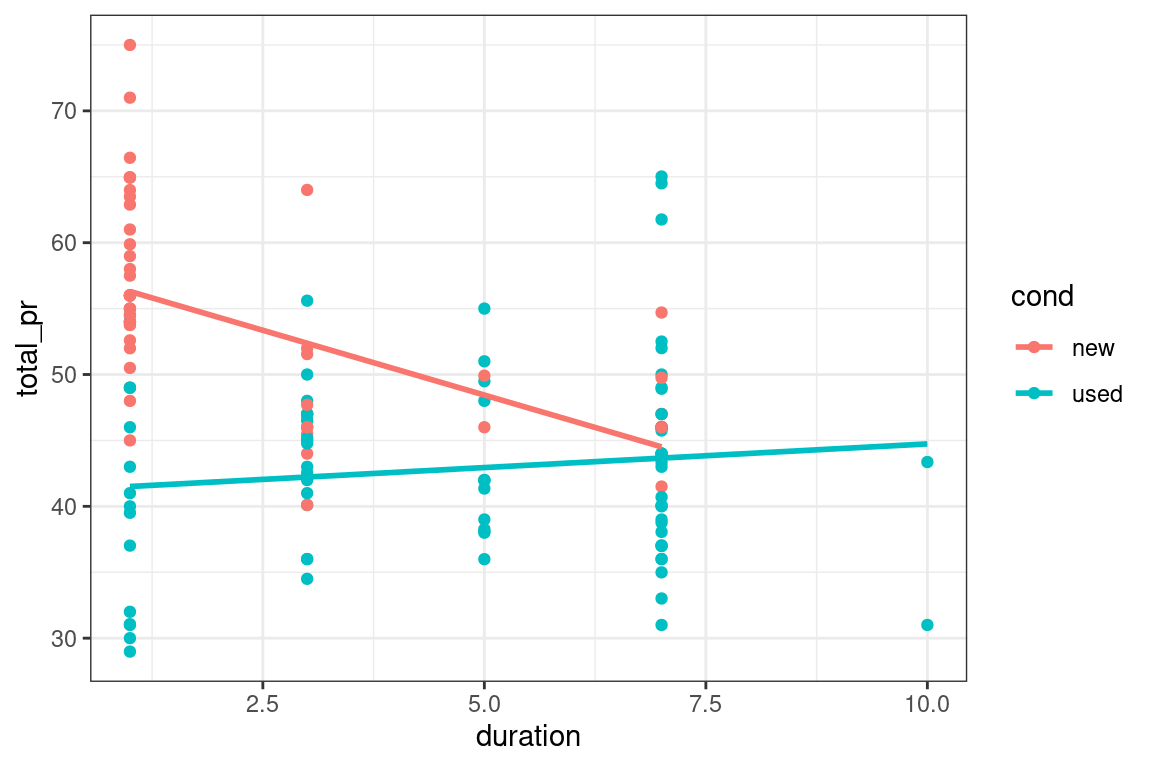
\includegraphics{CorrRegSC_files/figure-latex/unnamed-chunk-26-1} \end{center}

\begin{center}\rule{0.5\linewidth}{0.5pt}\end{center}

\hypertarget{uniqueness-of-least-squares-regression-line}{%
\section{Uniqueness of least squares regression line}\label{uniqueness-of-least-squares-regression-line}}

The least squares criterion implies that the slope of the regression line is unique. In practice, the slope is computed by R. In this exercise, you will experiment with trying to find the optimal value for the regression slope for weight as a function of height in the \texttt{bdims} dataset via trial-and-error.

To help, we've built a custom function for you called \texttt{add\_line()}, which takes a single argument: the proposed slope coefficient.

The \texttt{bdims} dataset is available in your workspace. Experiment with different values (to the nearest integer) of the \texttt{my\_slope} parameter until you find one that you think fits best.

\begin{Shaded}
\begin{Highlighting}[]
\CommentTok{# Estimate optimal value of my_slope}
\KeywordTok{add_line}\NormalTok{(}\DataTypeTok{my_slope =} \FloatTok{1.0}\NormalTok{)}
\end{Highlighting}
\end{Shaded}

\begin{center}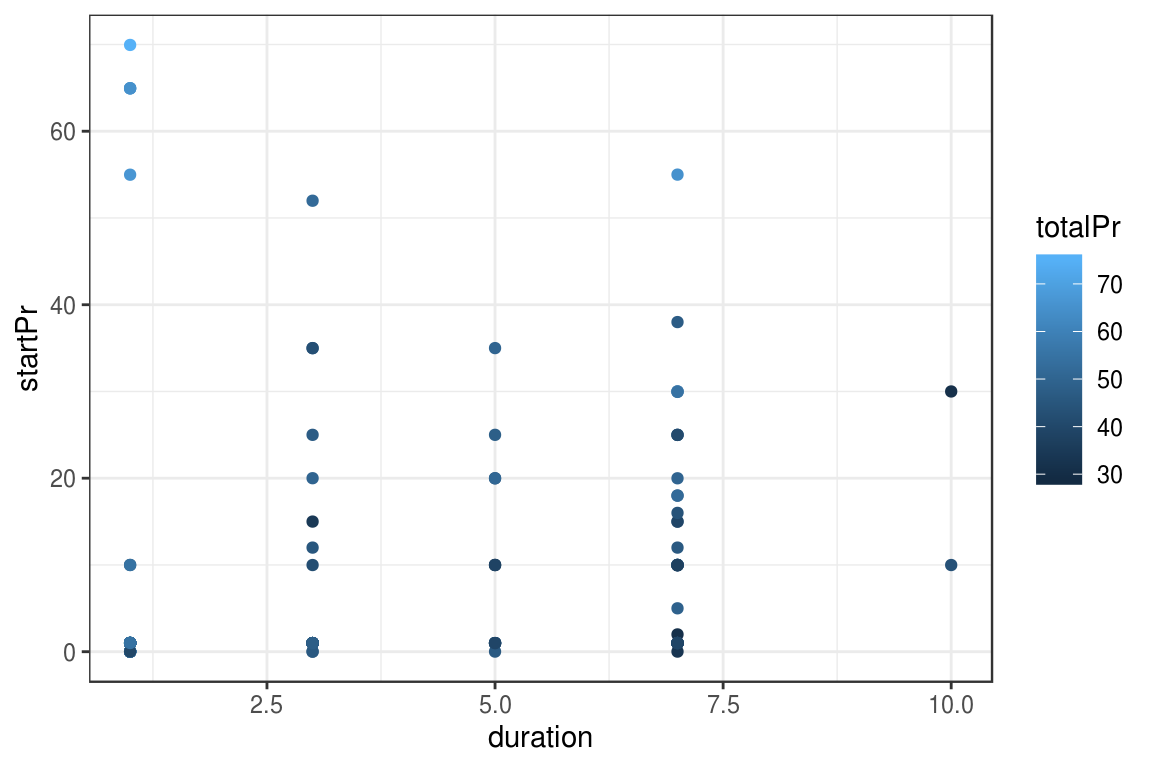
\includegraphics{CorrRegSC_files/figure-latex/unnamed-chunk-28-1} \end{center}

\begin{center}\rule{0.5\linewidth}{0.5pt}\end{center}

\hypertarget{regression-model-terminology}{%
\subsection*{Regression model terminology}\label{regression-model-terminology}}
\addcontentsline{toc}{subsection}{Regression model terminology}

Consider a linear regression model of the form:

\(Y=\beta_0+ \beta_1\cdot X + \varepsilon\), where \(\varepsilon \sim(0, \sigma_{\varepsilon})\)

The slope coefficient is:

\begin{itemize}
\item
  \(Y\)
\item
  \(\beta_0\)
\item
  \(\mathbf{\beta_1}\)
\item
  \(\varepsilon\)
\end{itemize}

\begin{center}\rule{0.5\linewidth}{0.5pt}\end{center}

\hypertarget{regression-model-output-terminology}{%
\subsection{Regression model output terminology}\label{regression-model-output-terminology}}

The fitted model for the poverty rate of U.S. counties as a function of high school graduation rate is:

\(\widehat{poverty} = 64.594 − 0.591 \cdot hs\_grad\)

In Hampshire County in western Massachusetts, the high school graduation rate is 92.4\%. These two facts imply that the poverty rate in Hampshire County is \_\_\_.

\begin{Shaded}
\begin{Highlighting}[]
\FloatTok{64.594} \OperatorTok{-}\StringTok{ }\FloatTok{0.591} \OperatorTok{*}\StringTok{ }\FloatTok{92.4}
\end{Highlighting}
\end{Shaded}

\begin{verbatim}
[1] 9.9856
\end{verbatim}

\begin{itemize}
\item
  exactly 11.7\%
\item
  exactly 10.0\%
\item
  \textbf{expected to be about 10.0\%}
\item
  expected to be about 11.7\%
\end{itemize}

\begin{center}\rule{0.5\linewidth}{0.5pt}\end{center}

\hypertarget{fitting-a-linear-model-by-hand}{%
\section{Fitting a linear model ``by hand''}\label{fitting-a-linear-model-by-hand}}

Recall the simple linear regression model:
\[Y=b_0 + b_1\cdot X\]
Two facts enable you to compute the slope \(b_1\) and intercept \(b_0\) of a simple linear regression model from some basic summary statistics.

First, the slope can be defined as:

\[b_1=r_{X,Y}\cdot \frac{s_Y}{s_X}\]
where \(r_{X,Y}\) represents the correlation (\texttt{cor()}) of \texttt{X} and \texttt{Y} and \(s_X\) and \(s_Y\) represent the standard deviation (\texttt{sd()}) of \texttt{X} and \texttt{Y}, respectively.

Second, the point \((\bar{x}, \bar{y})\) is always on the least squares regression line, where \(\bar{x}\) and \(\bar{y}\) denote the average of \(x\) and \(y\), respectively.

The \texttt{bdims\_summary} data frame contains all of the information you need to compute the slope and intercept of the least squares regression line for body weight (\texttt{Y}) as a function of height (\texttt{X}). You might need to do some algebra to solve for \(b_0\)!

\begin{Shaded}
\begin{Highlighting}[]
\NormalTok{bdims_summary <-}\StringTok{ }\NormalTok{bdims }\OperatorTok
\StringTok{    }\KeywordTok{summarize}\NormalTok{(}\DataTypeTok{N =} \KeywordTok{n}\NormalTok{(), }\DataTypeTok{r =} \KeywordTok{cor}\NormalTok{(wgt, hgt), }\DataTypeTok{mean_hgt =} \KeywordTok{mean}\NormalTok{(hgt),}
    \DataTypeTok{sd_hgt =} \KeywordTok{sd}\NormalTok{(hgt), }\DataTypeTok{mean_wgt =} \KeywordTok{mean}\NormalTok{(wgt), }\DataTypeTok{sd_wgt =} \KeywordTok{sd}\NormalTok{(wgt))}
\NormalTok{bdims_summary }
\end{Highlighting}
\end{Shaded}

\begin{verbatim}
# A tibble: 1 x 6
      N     r mean_hgt sd_hgt mean_wgt sd_wgt
  <int> <dbl>    <dbl>  <dbl>    <dbl>  <dbl>
1   507 0.717     171.   9.41     69.1   13.3
\end{verbatim}

\begin{Shaded}
\begin{Highlighting}[]
\CommentTok{# Add slope and intercept}
\NormalTok{bdims_summary }\OperatorTok
\StringTok{  }\KeywordTok{mutate}\NormalTok{(}\DataTypeTok{slope =}\NormalTok{ r}\OperatorTok{*}\NormalTok{sd_wgt}\OperatorTok{/}\NormalTok{sd_hgt, }
         \DataTypeTok{intercept =}\NormalTok{ mean_wgt }\OperatorTok{-}\StringTok{ }\NormalTok{slope}\OperatorTok{*}\NormalTok{mean_hgt)}
\end{Highlighting}
\end{Shaded}

\begin{verbatim}
# A tibble: 1 x 8
      N     r mean_hgt sd_hgt mean_wgt sd_wgt slope intercept
  <int> <dbl>    <dbl>  <dbl>    <dbl>  <dbl> <dbl>     <dbl>
1   507 0.717     171.   9.41     69.1   13.3  1.02     -105.
\end{verbatim}

\begin{center}\rule{0.5\linewidth}{0.5pt}\end{center}

\hypertarget{regression-to-the-mean}{%
\section{Regression to the mean}\label{regression-to-the-mean}}

Regression to the mean is a concept attributed to Sir Francis Galton. The basic idea is that extreme random observations will tend to be less extreme upon a second trial. This is simply due to chance alone. While ``regression to the mean'' and ``linear regression'' are not the same thing, we will examine them together in this exercise.

One way to see the effects of regression to the mean is to compare the heights of parents to their children's heights. While it is true that tall mothers and fathers tend to have tall children, those children tend to be less tall than their parents, relative to average. That is, fathers who are 3 inches taller than the average father tend to have children who may be taller than average, but by less than 3 inches.

The \texttt{Galton\_men} and \texttt{Galton\_women} datasets contain data originally collected by Galton himself in the 1880s on the heights of men and women, respectively, along with their parents' heights.

\begin{Shaded}
\begin{Highlighting}[]
\KeywordTok{download.file}\NormalTok{(}\StringTok{"http://www.randomservices.org/random/data/Galton.txt"}\NormalTok{, }\DataTypeTok{destfile =} \StringTok{"./Data/Galton.txt"}\NormalTok{)}
\NormalTok{Galton <-}\StringTok{ }\KeywordTok{read.table}\NormalTok{(}\StringTok{"./Data/Galton.txt"}\NormalTok{, }\DataTypeTok{header =} \OtherTok{TRUE}\NormalTok{)}
\NormalTok{Galton_men <-}\StringTok{ }\NormalTok{Galton }\OperatorTok
\StringTok{  }\KeywordTok{filter}\NormalTok{(Gender }\OperatorTok{==}\StringTok{ "M"}\NormalTok{)}
\NormalTok{Galton_women <-}\StringTok{ }\NormalTok{Galton }\OperatorTok\StringTok{ }
\StringTok{  }\KeywordTok{filter}\NormalTok{(Gender }\OperatorTok{==}\StringTok{ "F"}\NormalTok{)}
\end{Highlighting}
\end{Shaded}

Compare the slope of the regression line to the slope of the diagonal line. What does this tell you?

\hypertarget{exercise-9}{%
\subsection*{Exercise}\label{exercise-9}}
\addcontentsline{toc}{subsection}{Exercise}

\begin{itemize}
\tightlist
\item
  Create a scatterplot of the height of men as a function of their father's height. Add the simple linear regression line and a diagonal line (with slope equal to 1 and intercept equal to 0) to the plot.
\end{itemize}

\begin{Shaded}
\begin{Highlighting}[]
\CommentTok{# Height of children vs. height of father}
\KeywordTok{ggplot}\NormalTok{(}\DataTypeTok{data =}\NormalTok{ Galton_men, }\KeywordTok{aes}\NormalTok{(}\DataTypeTok{x =}\NormalTok{ Father, }\DataTypeTok{y =}\NormalTok{ Height)) }\OperatorTok{+}
\StringTok{  }\KeywordTok{geom_point}\NormalTok{(}\DataTypeTok{alpha =} \FloatTok{0.2}\NormalTok{) }\OperatorTok{+}\StringTok{ }
\StringTok{  }\KeywordTok{geom_abline}\NormalTok{(}\DataTypeTok{slope =} \DecValTok{1}\NormalTok{, }\DataTypeTok{intercept =} \DecValTok{0}\NormalTok{) }\OperatorTok{+}\StringTok{ }
\StringTok{  }\KeywordTok{geom_smooth}\NormalTok{(}\DataTypeTok{method =} \StringTok{"lm"}\NormalTok{, }\DataTypeTok{se =} \OtherTok{FALSE}\NormalTok{) }\OperatorTok{+}\StringTok{ }
\StringTok{  }\KeywordTok{theme_bw}\NormalTok{()}
\end{Highlighting}
\end{Shaded}

\begin{verbatim}
`geom_smooth()` using formula 'y ~ x'
\end{verbatim}

\begin{center}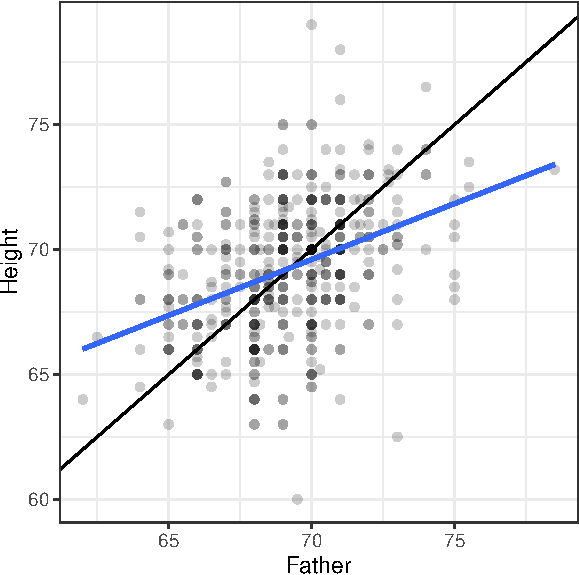
\includegraphics{CorrRegSC_files/figure-latex/unnamed-chunk-32-1} \end{center}

\begin{itemize}
\tightlist
\item
  Create a scatterplot of the height of women as a function of their mother's height. Add the simple linear regression line and a diagonal line to the plot.
\end{itemize}

\begin{Shaded}
\begin{Highlighting}[]
\CommentTok{# Height of children vs. height of mother}
\KeywordTok{ggplot}\NormalTok{(}\DataTypeTok{data =}\NormalTok{ Galton_women, }\KeywordTok{aes}\NormalTok{(}\DataTypeTok{x =}\NormalTok{ Mother, }\DataTypeTok{y =}\NormalTok{ Height)) }\OperatorTok{+}
\StringTok{  }\KeywordTok{geom_point}\NormalTok{(}\DataTypeTok{alpha =} \FloatTok{0.2}\NormalTok{) }\OperatorTok{+}\StringTok{ }
\StringTok{  }\KeywordTok{geom_abline}\NormalTok{(}\DataTypeTok{slope =} \DecValTok{1}\NormalTok{, }\DataTypeTok{intercept =} \DecValTok{0}\NormalTok{) }\OperatorTok{+}\StringTok{ }
\StringTok{  }\KeywordTok{geom_smooth}\NormalTok{(}\DataTypeTok{method =} \StringTok{"lm"}\NormalTok{, }\DataTypeTok{se =} \OtherTok{FALSE}\NormalTok{) }\OperatorTok{+}\StringTok{ }
\StringTok{  }\KeywordTok{theme_bw}\NormalTok{()}
\end{Highlighting}
\end{Shaded}

\begin{verbatim}
`geom_smooth()` using formula 'y ~ x'
\end{verbatim}

\begin{center}
\includegraphics{CorrRegSC_files/figure-latex/unnamed-chunk-33-1} \end{center}

\begin{center}\rule{0.5\linewidth}{0.5pt}\end{center}

\hypertarget{regression-in-the-parlance-of-our-time}{%
\subsection*{``Regression'' in the parlance of our time}\label{regression-in-the-parlance-of-our-time}}
\addcontentsline{toc}{subsection}{``Regression'' in the parlance of our time}

In an opinion piece about nepotism \href{https://www.nytimes.com/2015/03/22/opinion/sunday/seth-stephens-davidowitz-just-how-nepotistic-are-we.html}{published in The New York Times in 2015}, economist Seth Stephens-Davidowitz wrote that:

\begin{quote}
``Regression to the mean is so powerful that once-in-a-generation talent basically never sires once-in-a-generation talent. It explains why Michael Jordan's sons were middling college basketball players and Jakob Dylan wrote two good songs. It is why there are no American parent-child pairs among Hall of Fame players in any major professional sports league.''
\end{quote}

The author is arguing that\ldots{}

\begin{itemize}
\item
  Because of regression to the mean, an outstanding basketball player is likely to have sons that are as good at basketball as him.
\item
  Because of regression to the mean, an outstanding basketball player is likely to have sons that are not good at basketball.
\item
  \textbf{Because of regression to the mean, an outstanding basketball player is likely to have sons that are good at basketball, but not as good as him.}
\item
  Linear regression is incapable of evaluating musical or athletic talent.
\end{itemize}

\begin{center}\rule{0.5\linewidth}{0.5pt}\end{center}

\hypertarget{interpreting-regression-models}{%
\chapter{Interpreting regression models}\label{interpreting-regression-models}}

This chapter looks at how to interpret the coefficients in a regression model.

\hypertarget{interpretation-of-coefficients}{%
\subsection*{Interpretation of coefficients}\label{interpretation-of-coefficients}}
\addcontentsline{toc}{subsection}{Interpretation of coefficients}

Recall that the fitted model for the poverty rare of U.S. countries as a function of high school graduation rate is:

\begin{equation}
\widehat{poverty} = 64.594 - 0.591\cdot {hs\_grad}
\end{equation}

Which of the following equations is the correct interpretation of the slope coefficient?

\begin{itemize}
\tightlist
\item
  Among U.S. counties, each additional percentage point increase in the poverty rate is associated with about a 0.591 percentage point decrease in the high school graduation rate.
\item
  \textbf{Among U.S. counties, each additional percentage point increase in the high school graduation rate is associated with about a 0.591 percentage point decrease in the poverty rate.}
\item
  Among U.S. counties, each additional percentage point increase in the high school graduation rate is associated with about a 0.591 percentage point increase in the poverty rate.
\item
  Among U.S. counties, a 1\% increase in the high school graduation rate is associated with about a 0.591\% decrease in the poverty rate.
\end{itemize}

\begin{center}\rule{0.5\linewidth}{0.5pt}\end{center}

\hypertarget{interpretation-in-context}{%
\subsection*{Interpretation in context}\label{interpretation-in-context}}
\addcontentsline{toc}{subsection}{Interpretation in context}

A politician interpreting the relationship between poverty rates and high school graduation rates implores his constituents:

If we can lower the poverty rate by 59\%, we'll double the high school graduate rate in our county (i.e.~raise it by 100\%).

Which of the following mistakes in interpretation has the politician made?

\begin{itemize}
\item
  Implying that the regression model establishes a cause-and-effect relationship.
\item
  Switching the role of the response and explanatory variables.
\item
  Confusing percentage change with percentage point change.
\item
  \textbf{All of the above.}
\item
  None of the above.
\end{itemize}

\begin{center}\rule{0.5\linewidth}{0.5pt}\end{center}

\hypertarget{fitting-simple-linear-models}{%
\section{Fitting simple linear models}\label{fitting-simple-linear-models}}

While the \texttt{geom\_smooth(method\ =\ "lm")} function is useful for drawing linear models on a scatterplot, it doesn't actually return the characteristics of the model. As suggested by that syntax, however, the function that creates linear models is \texttt{lm()}. This function generally takes two arguments:

\begin{itemize}
\item
  A \texttt{formula} that specifies the model
\item
  A \texttt{data} argument for the data frame that contains the data you want to fit to the model
\end{itemize}

The \texttt{lm()} function return a model object having class \texttt{"lm"}. This object contains lots of information about your regression model, including the data used to fit the model, the specification of the model, the fitted values and residuals, etc.

\begin{center}\rule{0.5\linewidth}{0.5pt}\end{center}

\hypertarget{excercise}{%
\subsection*{Excercise}\label{excercise}}
\addcontentsline{toc}{subsection}{Excercise}

\begin{itemize}
\tightlist
\item
  Using the \texttt{bdims} dataset, create a linear model for the weight of people as a function of their height.
\end{itemize}

\begin{Shaded}
\begin{Highlighting}[]
\KeywordTok{library}\NormalTok{(openintro)}
\CommentTok{# Linear model for weight as a function of height}
\KeywordTok{lm}\NormalTok{(wgt }\OperatorTok{~}\StringTok{ }\NormalTok{hgt, }\DataTypeTok{data =}\NormalTok{ bdims)}
\end{Highlighting}
\end{Shaded}

\begin{verbatim}

Call:
lm(formula = wgt ~ hgt, data = bdims)

Coefficients:
(Intercept)          hgt  
   -105.011        1.018  
\end{verbatim}

\begin{itemize}
\tightlist
\item
  Using the \texttt{mlbBat10} dataset, create a linear model for \texttt{SLG} as a function of \texttt{OBP}.
\end{itemize}

\begin{Shaded}
\begin{Highlighting}[]
\CommentTok{# Linear model for SLG as a function of OBP}
\KeywordTok{lm}\NormalTok{(slg }\OperatorTok{~}\StringTok{ }\NormalTok{obp, }\DataTypeTok{data =}\NormalTok{ mlbbat10)}
\end{Highlighting}
\end{Shaded}

\begin{verbatim}

Call:
lm(formula = slg ~ obp, data = mlbbat10)

Coefficients:
(Intercept)          obp  
   0.009407     1.110323  
\end{verbatim}

*Using the \texttt{mammals} dataset, create a linear model for the body weight of mammals as a function of their brain weight, after taking the natural log of both variables.

\begin{Shaded}
\begin{Highlighting}[]
\CommentTok{# Log-linear model for body weight as a function of brain weight}
\KeywordTok{lm}\NormalTok{(}\KeywordTok{log}\NormalTok{(body_wt) }\OperatorTok{~}\StringTok{ }\KeywordTok{log}\NormalTok{(brain_wt), }\DataTypeTok{data =}\NormalTok{ mammals)}
\end{Highlighting}
\end{Shaded}

\begin{verbatim}

Call:
lm(formula = log(body_wt) ~ log(brain_wt), data = mammals)

Coefficients:
  (Intercept)  log(brain_wt)  
       -2.509          1.225  
\end{verbatim}

\begin{center}\rule{0.5\linewidth}{0.5pt}\end{center}

\hypertarget{units-and-scale}{%
\subsection*{Units and scale}\label{units-and-scale}}
\addcontentsline{toc}{subsection}{Units and scale}

In the previous examples, we fit two regression models:

\begin{equation}
\widehat{wgt} = −105.011 + 1.018 \cdot hgt
\end{equation}

and

\begin{equation}
\widehat{SLG}= 0.009 + 1.110 \cdot OBP
\end{equation}

Which of the following statements is \textbf{incorrect}?

\begin{itemize}
\item
  A person who is 170 cm tall is expected to weigh about 68 kg.
\item
  \textbf{Because the slope coefficient for OBP is larger (1.110) than the slope coefficient for hgt (1.018), we can conclude that the association between OBP and SLG is stronger than the association between height and weight.}
\item
  None of the above.
\end{itemize}

\begin{center}\rule{0.5\linewidth}{0.5pt}\end{center}

\hypertarget{the-lm-summary-output}{%
\section{The lm summary output}\label{the-lm-summary-output}}

An \texttt{lm} object contains a host of information about the regression model that you fit. There are various ways of extracting different pieces of information.

The \texttt{coef()} function displays only the values of the coefficients. Conversely, the \texttt{summary()} function displays not only that information, but a bunch of other information, including the associated standard error and p-value for each coefficient, the, \(R^2\) adjusted \(R^2\), and the residual standard error. The summary of an \texttt{"lm"} object in R is very similar to the output you would see in other statistical computing environments (e.g.~Stata, SPSS, etc.)

\begin{center}\rule{0.5\linewidth}{0.5pt}\end{center}

\hypertarget{excercise-1}{%
\subsection*{Excercise}\label{excercise-1}}
\addcontentsline{toc}{subsection}{Excercise}

We have already created the mod object, a linear model for the weight of individuals as a function of their height, using the \texttt{bdims} dataset and the code

\begin{Shaded}
\begin{Highlighting}[]
\NormalTok{mod <-}\StringTok{ }\KeywordTok{lm}\NormalTok{(wgt }\OperatorTok{~}\StringTok{ }\NormalTok{hgt, }\DataTypeTok{data =}\NormalTok{ bdims)}
\end{Highlighting}
\end{Shaded}

Now, you will:

\begin{itemize}
\tightlist
\item
  Use \texttt{coef()} to display the coefficients of \texttt{mod}.
\end{itemize}

\begin{Shaded}
\begin{Highlighting}[]
\NormalTok{mod <-}\StringTok{ }\KeywordTok{lm}\NormalTok{(wgt }\OperatorTok{~}\StringTok{ }\NormalTok{hgt, }\DataTypeTok{data =}\NormalTok{ bdims)}
\CommentTok{# Show the coefficients}
\KeywordTok{coef}\NormalTok{(mod)}
\end{Highlighting}
\end{Shaded}

\begin{verbatim}
(Intercept)         hgt 
-105.011254    1.017617 
\end{verbatim}

\begin{itemize}
\tightlist
\item
  Use \texttt{summary()} to display the full regression output of \texttt{mod()}.
\end{itemize}

\begin{Shaded}
\begin{Highlighting}[]
\KeywordTok{summary}\NormalTok{(mod)}
\end{Highlighting}
\end{Shaded}

\begin{verbatim}

Call:
lm(formula = wgt ~ hgt, data = bdims)

Residuals:
    Min      1Q  Median      3Q     Max 
-18.743  -6.402  -1.231   5.059  41.103 

Coefficients:
              Estimate Std. Error t value Pr(>|t|)    
(Intercept) -105.01125    7.53941  -13.93   <2e-16 ***
hgt            1.01762    0.04399   23.14   <2e-16 ***
---
Signif. codes:  0 '***' 0.001 '**' 0.01 '*' 0.05 '.' 0.1 ' ' 1

Residual standard error: 9.308 on 505 degrees of freedom
Multiple R-squared:  0.5145,    Adjusted R-squared:  0.5136 
F-statistic: 535.2 on 1 and 505 DF,  p-value: < 2.2e-16
\end{verbatim}

\begin{center}\rule{0.5\linewidth}{0.5pt}\end{center}

\hypertarget{fitted-values-and-residuals}{%
\section{Fitted values and residuals}\label{fitted-values-and-residuals}}

Once you have fit a regression model, you are often interested in the fitted values \((\hat{y_i})\) and the residuals \(({e_i})\), where \(i\) indexes the observations. Recall that:
\begin{equation}
e_i = y_i - \hat{y}_i
\end{equation}
The least squares fitting procedure guarantees that the mean of the residuals is zero (n.b., numerical instability may result in the computed values not being exactly zero). At the same time, the mean of the fitted values must equal the mean of the response variable.

In this exercise, we will confirm these two mathematical facts by accessing the fitted values and residuals with the \texttt{fitted.values()} and \texttt{residuals()} functions, respectively, for the following model:

\begin{Shaded}
\begin{Highlighting}[]
\NormalTok{mod <-}\StringTok{ }\KeywordTok{lm}\NormalTok{(wgt }\OperatorTok{~}\StringTok{ }\NormalTok{hgt, }\DataTypeTok{data =}\NormalTok{ bdims)}
\end{Highlighting}
\end{Shaded}

\begin{center}\rule{0.5\linewidth}{0.5pt}\end{center}

\hypertarget{exercise-10}{%
\subsection*{Exercise}\label{exercise-10}}
\addcontentsline{toc}{subsection}{Exercise}

\begin{itemize}
\tightlist
\item
  Confirm that the mean of the body weights equals the mean of the fitted values of \texttt{mod}.
\end{itemize}

\begin{Shaded}
\begin{Highlighting}[]
\CommentTok{# Mean of weights equal to mean of fitted values?}
\KeywordTok{mean}\NormalTok{(bdims}\OperatorTok{$}\NormalTok{wgt) }\OperatorTok{==}\StringTok{ }\KeywordTok{mean}\NormalTok{(}\KeywordTok{fitted.values}\NormalTok{(mod))}
\end{Highlighting}
\end{Shaded}

\begin{verbatim}
[1] TRUE
\end{verbatim}

\begin{itemize}
\tightlist
\item
  Compute the mean of the residuals of \texttt{mod}.
\end{itemize}

\begin{Shaded}
\begin{Highlighting}[]
\KeywordTok{mean}\NormalTok{(}\KeywordTok{resid}\NormalTok{(mod))}
\end{Highlighting}
\end{Shaded}

\begin{verbatim}
[1] -3.665467e-16
\end{verbatim}

\begin{center}\rule{0.5\linewidth}{0.5pt}\end{center}

\hypertarget{tidying-your-linear-model}{%
\section{Tidying your linear model}\label{tidying-your-linear-model}}

As you fit a regression model, there are some quantities (e.g.~\(R^2\)) hat apply to the model as a whole, while others apply to each observation (e.g.~\(\hat{y_i}\)). If there are several of these per-observation quantities, it is sometimes convenient to attach them to the original data as new variables.

The \texttt{augment()} function from the \texttt{broom} package does exactly this. It takes a model object as an argument and returns a data frame that contains the data on which the model was fit, along with several quantities specific to the regression model, including the fitted values, residuals, leverage scores, and standardized residuals.

\begin{center}\rule{0.5\linewidth}{0.5pt}\end{center}

\hypertarget{excercise-2}{%
\subsection*{Excercise}\label{excercise-2}}
\addcontentsline{toc}{subsection}{Excercise}

The same linear model from the last exercise, \texttt{mod}, is available in your workspace.

\begin{itemize}
\tightlist
\item
  Load the \texttt{broom} package.
\end{itemize}

\begin{Shaded}
\begin{Highlighting}[]
\CommentTok{# Load broom}
\KeywordTok{library}\NormalTok{(broom)}
\end{Highlighting}
\end{Shaded}

\begin{itemize}
\tightlist
\item
  Create a new data frame called \texttt{bdims\_tidy} that is the augmentation of the \texttt{mod} linear model.
\end{itemize}

\begin{Shaded}
\begin{Highlighting}[]
\CommentTok{# Create bdims_tidy}
\NormalTok{bdims_tidy <-}\StringTok{ }\KeywordTok{augment}\NormalTok{(mod)}
\end{Highlighting}
\end{Shaded}

\begin{itemize}
\tightlist
\item
  View the \texttt{bdims\_tidy} data frame using \texttt{glimpse()}.
\end{itemize}

\begin{Shaded}
\begin{Highlighting}[]
\CommentTok{# Glimpse the resulting data frame}
\KeywordTok{glimpse}\NormalTok{(bdims_tidy)}
\end{Highlighting}
\end{Shaded}

\begin{verbatim}
Rows: 507
Columns: 8
$ wgt        <dbl> 65.6, 71.8, 80.7, 72.6, 78.8, 74.8, 86.4, 78.4, 62.0, 81...
$ hgt        <dbl> 174.0, 175.3, 193.5, 186.5, 187.2, 181.5, 184.0, 184.5, ...
$ .fitted    <dbl> 72.05406, 73.37697, 91.89759, 84.77427, 85.48661, 79.686...
$ .resid     <dbl> -6.4540648, -1.5769666, -11.1975919, -12.1742745, -6.686...
$ .hat       <dbl> 0.002154570, 0.002358152, 0.013133942, 0.007238576, 0.00...
$ .sigma     <dbl> 9.312824, 9.317005, 9.303732, 9.301360, 9.312471, 9.3147...
$ .cooksd    <dbl> 5.201807e-04, 3.400330e-05, 9.758463e-03, 6.282074e-03, ...
$ .std.resid <dbl> -0.69413418, -0.16961994, -1.21098084, -1.31269063, -0.7...
\end{verbatim}

\begin{center}\rule{0.5\linewidth}{0.5pt}\end{center}

\hypertarget{making-predictions}{%
\section{Making predictions}\label{making-predictions}}

The \texttt{fitted.values()} function or the \texttt{augment()}-ed data frame provides us with the fitted values for the observations that were in the original data. However, once we have fit the model, we may want to compute expected values for observations that were not present in the data on which the model was fit. These types of predictions are called out-of-sample.

The \texttt{ben} data frame contains a height and weight observation for one person.

\begin{Shaded}
\begin{Highlighting}[]
\NormalTok{ben <-}\StringTok{ }\KeywordTok{data.frame}\NormalTok{(}\DataTypeTok{wgt =} \FloatTok{74.8}\NormalTok{, }\DataTypeTok{hgt =} \FloatTok{182.8}\NormalTok{)}
\end{Highlighting}
\end{Shaded}

The \texttt{mod} object contains the fitted model for weight as a function of height for the observations in the \texttt{bdims} dataset. We can use the \texttt{predict()} function to generate expected values for the weight of new individuals. We must pass the data frame of new observations through the \texttt{newdata} argument.

\begin{center}\rule{0.5\linewidth}{0.5pt}\end{center}

\hypertarget{excercise-3}{%
\subsection*{Excercise}\label{excercise-3}}
\addcontentsline{toc}{subsection}{Excercise}

The same linear model, \texttt{mod}, is defined in your workspace.

\begin{itemize}
\tightlist
\item
  Print \texttt{ben} to the console.
\end{itemize}

\begin{Shaded}
\begin{Highlighting}[]
\CommentTok{# Print ben}
\NormalTok{ben}
\end{Highlighting}
\end{Shaded}

\begin{verbatim}
   wgt   hgt
1 74.8 182.8
\end{verbatim}

\begin{itemize}
\tightlist
\item
  Use \texttt{predict()} with the \texttt{newdata} argument to compute the expected weight of the individual in the \texttt{ben} data frame.
\end{itemize}

\begin{Shaded}
\begin{Highlighting}[]
\CommentTok{# Predict the weight of ben}
\KeywordTok{predict}\NormalTok{(mod, }\DataTypeTok{newdata =}\NormalTok{ ben)}
\end{Highlighting}
\end{Shaded}

\begin{verbatim}
       1 
81.00909 
\end{verbatim}

\textbf{Note} that the data frame \texttt{ben} has variables with the exact same names as those in the fitted model.

\begin{center}\rule{0.5\linewidth}{0.5pt}\end{center}

\hypertarget{adding-a-regression-line-to-a-plot-manually}{%
\section{Adding a regression line to a plot manually}\label{adding-a-regression-line-to-a-plot-manually}}

The \texttt{geom\_smooth()} function makes it easy to add a simple linear regression line to a scatterplot of the corresponding variables. And in fact, there are more complicated regression models that can be visualized in the data space with \texttt{geom\_smooth()}. However, there may still be times when we will want to add regression lines to our scatterplot manually. To do this, we will use the \texttt{geom\_abline()} function, which takes slope and intercept arguments. Naturally, we have to compute those values ahead of time, but we already saw how to do this (e.g.~using \texttt{coef()}).

The \texttt{coefs} data frame contains the model estimates retrieved from \texttt{coef()}. Passing this to \texttt{geom\_abline()} as the data argument will enable you to draw a straight line on your scatterplot.

\begin{center}\rule{0.5\linewidth}{0.5pt}\end{center}

\hypertarget{excercise-4}{%
\subsection*{Excercise}\label{excercise-4}}
\addcontentsline{toc}{subsection}{Excercise}

Use \texttt{geom\_abline()} to add a line defined in the \texttt{coefs} data frame to a scatterplot of weight vs.~height for individuals in the \texttt{bdims} dataset.

\begin{Shaded}
\begin{Highlighting}[]
\KeywordTok{coef}\NormalTok{(mod)}
\end{Highlighting}
\end{Shaded}

\begin{verbatim}
(Intercept)         hgt 
-105.011254    1.017617 
\end{verbatim}

\begin{Shaded}
\begin{Highlighting}[]
\NormalTok{coefs <-}\StringTok{ }\KeywordTok{data.frame}\NormalTok{(}\DataTypeTok{intercept =} \DecValTok{-105}\NormalTok{, }\DataTypeTok{slope =} \FloatTok{1.018}\NormalTok{)}
\NormalTok{coefs}
\end{Highlighting}
\end{Shaded}

\begin{verbatim}
  intercept slope
1      -105 1.018
\end{verbatim}

\begin{Shaded}
\begin{Highlighting}[]
\CommentTok{# Add the line to the scatterplot}
\KeywordTok{ggplot}\NormalTok{(}\DataTypeTok{data =}\NormalTok{ bdims, }\KeywordTok{aes}\NormalTok{(}\DataTypeTok{x =}\NormalTok{ hgt, }\DataTypeTok{y =}\NormalTok{ wgt)) }\OperatorTok{+}
\StringTok{  }\KeywordTok{geom_point}\NormalTok{(}\DataTypeTok{alpha =} \FloatTok{0.5}\NormalTok{) }\OperatorTok{+}\StringTok{ }
\StringTok{  }\KeywordTok{theme_bw}\NormalTok{() }\OperatorTok{+}\StringTok{ }
\StringTok{  }\KeywordTok{geom_abline}\NormalTok{(}\DataTypeTok{data =}\NormalTok{ coefs, }
              \KeywordTok{aes}\NormalTok{(}\DataTypeTok{intercept =}\NormalTok{ intercept, }\DataTypeTok{slope =}\NormalTok{ slope),  }
              \DataTypeTok{color =} \StringTok{"dodgerblue"}\NormalTok{)}
\end{Highlighting}
\end{Shaded}

\begin{center}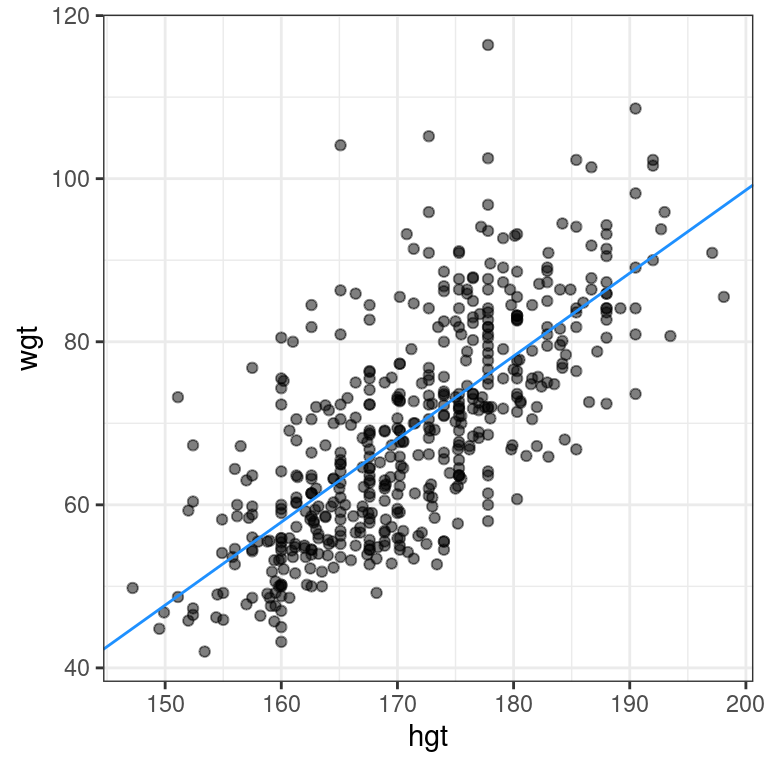
\includegraphics{CorrRegSC_files/figure-latex/unnamed-chunk-52-1} \end{center}

\begin{center}\rule{0.5\linewidth}{0.5pt}\end{center}

\hypertarget{model-fit}{%
\chapter{Model Fit}\label{model-fit}}

In this final chapter, you'll learn how to assess the ``fit'' of a simple linear regression model.

\hypertarget{rmse}{%
\subsection*{RMSE}\label{rmse}}
\addcontentsline{toc}{subsection}{RMSE}

The residual standard error reported for the regression model for poverty rate of U.S. counties in terms of high school graduation rate is 4.67. What does this mean?

\begin{itemize}
\item
  \textbf{The typical difference between the observed poverty rate and the poverty rate predicted by the model is about 4.67 percentage points.}
\item
  The typical difference between the observed poverty rate and the poverty rate predicted by the model is about 4.67\%.
\end{itemize}

*The model explains about 4.67\% of the variability in poverty rate among counties.

\begin{itemize}
\tightlist
\item
  The model correctly predicted the poverty rate of 4.67\% of the counties.
\end{itemize}

\begin{center}\rule{0.5\linewidth}{0.5pt}\end{center}

\hypertarget{standard-error-of-residuals}{%
\section{Standard error of residuals}\label{standard-error-of-residuals}}

One way to assess strength of fit is to consider how far off the model is for a typical case. That is, for some observations, the fitted value will be very close to the actual value, while for others it will not. The magnitude of a typical residual can give us a sense of generally how close our estimates are.

However, recall that some of the residuals are positive, while others are negative. In fact, it is guaranteed by the least squares fitting procedure that the mean of the residuals is zero. Thus, it makes more sense to compute the square root of the mean squared residual, or root mean squared error (RMSE). R calls this quantity the \emph{residual standard error}.

To make this estimate unbiased, you have to divide the sum of the squared residuals by the degrees of freedom in the model. Thus,

\begin{equation}
RMSE = \sqrt{\frac{\sum_i e_i^2}{d.f.}} = \sqrt{\frac{SSE}{d.f.}}
\end{equation}

You can recover the residuals from \texttt{mod} with \texttt{residuals()}, and the degrees of freedom with \texttt{df.residual()}.

\begin{center}\rule{0.5\linewidth}{0.5pt}\end{center}

\hypertarget{exercise-11}{%
\subsection*{Exercise}\label{exercise-11}}
\addcontentsline{toc}{subsection}{Exercise}

*View a \texttt{summary()} of \texttt{mod}.

\begin{Shaded}
\begin{Highlighting}[]
\CommentTok{# View summary of model}
\KeywordTok{summary}\NormalTok{(mod)}
\end{Highlighting}
\end{Shaded}

\begin{verbatim}

Call:
lm(formula = wgt ~ hgt, data = bdims)

Residuals:
    Min      1Q  Median      3Q     Max 
-18.743  -6.402  -1.231   5.059  41.103 

Coefficients:
              Estimate Std. Error t value Pr(>|t|)    
(Intercept) -105.01125    7.53941  -13.93   <2e-16 ***
hgt            1.01762    0.04399   23.14   <2e-16 ***
---
Signif. codes:  0 '***' 0.001 '**' 0.01 '*' 0.05 '.' 0.1 ' ' 1

Residual standard error: 9.308 on 505 degrees of freedom
Multiple R-squared:  0.5145,    Adjusted R-squared:  0.5136 
F-statistic: 535.2 on 1 and 505 DF,  p-value: < 2.2e-16
\end{verbatim}

\begin{itemize}
\tightlist
\item
  Compute the mean of the \texttt{residuals()} and verify that it is approximately zero.
\end{itemize}

\begin{Shaded}
\begin{Highlighting}[]
\CommentTok{# Compute the mean of the residuals}
\KeywordTok{mean}\NormalTok{(}\KeywordTok{resid}\NormalTok{(mod))}
\end{Highlighting}
\end{Shaded}

\begin{verbatim}
[1] -3.665467e-16
\end{verbatim}

\begin{itemize}
\tightlist
\item
  Use \texttt{residuals()} and \texttt{df.residual()} to compute the root mean squared error (RMSE), a.k.a. \emph{residual standard error}.
\end{itemize}

\begin{Shaded}
\begin{Highlighting}[]
\CommentTok{# Compute RMSE}
\KeywordTok{sqrt}\NormalTok{(}\KeywordTok{sum}\NormalTok{(}\KeywordTok{residuals}\NormalTok{(mod)}\OperatorTok{^}\DecValTok{2}\NormalTok{) }\OperatorTok{/}\StringTok{ }\KeywordTok{df.residual}\NormalTok{(mod))}
\end{Highlighting}
\end{Shaded}

\begin{verbatim}
[1] 9.30804
\end{verbatim}

\begin{center}\rule{0.5\linewidth}{0.5pt}\end{center}

\hypertarget{assessing-simple-linear-model-fit}{%
\section{Assessing simple linear model fit}\label{assessing-simple-linear-model-fit}}

Recall that the coefficient of determination (\(R^2\)), can be computed as

\begin{equation}
R^2 = 1 − \frac{SSE}{SST} = 1 − \frac{Var(e)}{Var(y)},
\end{equation}

where \(e\) is the vector of residuals and \(y\) is the response variable. This gives us the interpretation of \(R^2\) as the percentage of the variability in the response that is explained by the model, since the residuals are the part of that variability that remains unexplained by the model.

\begin{center}\rule{0.5\linewidth}{0.5pt}\end{center}

The \texttt{bdims\_tidy} data frame is the result of \texttt{augment()}-ing the \texttt{bdims} data frame with the mod for wgt as a function of \texttt{hgt}.

\begin{Shaded}
\begin{Highlighting}[]
\NormalTok{bdims_tidy <-}\StringTok{ }\KeywordTok{augment}\NormalTok{(mod)}
\end{Highlighting}
\end{Shaded}

\begin{itemize}
\tightlist
\item
  Use the \texttt{summary()} function to view the full results of mod.
\end{itemize}

\begin{Shaded}
\begin{Highlighting}[]
\CommentTok{# View model summary}
\KeywordTok{summary}\NormalTok{(mod)}
\end{Highlighting}
\end{Shaded}

\begin{verbatim}

Call:
lm(formula = wgt ~ hgt, data = bdims)

Residuals:
    Min      1Q  Median      3Q     Max 
-18.743  -6.402  -1.231   5.059  41.103 

Coefficients:
              Estimate Std. Error t value Pr(>|t|)    
(Intercept) -105.01125    7.53941  -13.93   <2e-16 ***
hgt            1.01762    0.04399   23.14   <2e-16 ***
---
Signif. codes:  0 '***' 0.001 '**' 0.01 '*' 0.05 '.' 0.1 ' ' 1

Residual standard error: 9.308 on 505 degrees of freedom
Multiple R-squared:  0.5145,    Adjusted R-squared:  0.5136 
F-statistic: 535.2 on 1 and 505 DF,  p-value: < 2.2e-16
\end{verbatim}

\begin{itemize}
\tightlist
\item
  Use the \texttt{bdims\_tidy} data frame to compute the \(R^2\) of \texttt{mod} manually using the formula above, by computing the ratio of the variance of the residuals to the variance of the response variable.
\end{itemize}

\begin{Shaded}
\begin{Highlighting}[]
\NormalTok{bdims_tidy }\OperatorTok
\StringTok{  }\KeywordTok{summarize}\NormalTok{(}\DataTypeTok{var_y =} \KeywordTok{var}\NormalTok{(wgt), }\DataTypeTok{var_e =} \KeywordTok{var}\NormalTok{(.resid)) }\OperatorTok
\StringTok{  }\KeywordTok{mutate}\NormalTok{(}\DataTypeTok{R_squared =} \DecValTok{1} \OperatorTok{-}\StringTok{ }\NormalTok{var_e}\OperatorTok{/}\NormalTok{var_y)}
\end{Highlighting}
\end{Shaded}

\begin{verbatim}
# A tibble: 1 x 3
  var_y var_e R_squared
  <dbl> <dbl>     <dbl>
1  178.  86.5     0.515
\end{verbatim}

This means that 51.4\% of the variability in weight is explained by height.

\begin{center}\rule{0.5\linewidth}{0.5pt}\end{center}

\hypertarget{interpretation-of-r2}{%
\subsection*{\texorpdfstring{Interpretation of \(R^2\)}{Interpretation of R\^{}2}}\label{interpretation-of-r2}}
\addcontentsline{toc}{subsection}{Interpretation of \(R^2\)}

The \(R^2\) reported for the regression model for poverty rate of U.S. counties in terms of high school graduation rate is 0.464.

\begin{Shaded}
\begin{Highlighting}[]
\KeywordTok{lm}\NormalTok{(}\DataTypeTok{formula =}\NormalTok{ poverty }\OperatorTok{~}\StringTok{ }\NormalTok{hs_grad, }\DataTypeTok{data =}\NormalTok{ countyComplete) }\OperatorTok
\StringTok{  }\KeywordTok{summary}\NormalTok{()}
\end{Highlighting}
\end{Shaded}

How should this result be interpreted?

\begin{center}\rule{0.5\linewidth}{0.5pt}\end{center}

\begin{itemize}
\item
  46.4\% of the variability in high school graduate rate among U.S. counties can be explained by poverty rate.
\item
  \textbf{46.4\% of the variability in poverty rate among U.S. counties can be explained by high school graduation rate.}
\item
  This model is 46.4\% effective.
\item
  The correlation between poverty rate and high school graduation rate is 0.464.
\end{itemize}

\begin{center}\rule{0.5\linewidth}{0.5pt}\end{center}

\hypertarget{linear-vs.-average}{%
\section{Linear vs.~average}\label{linear-vs.-average}}

The \(R^2\) gives us a numerical measurement of the strength of fit relative to a null model based on the average of the response variable:

\begin{equation}
\hat{y}=\bar{y}
\end{equation}

This model has an \(R^2\) of zero because \(SSE = SST\). That is, since the fitted values (\(\hat{y}_{null}\)) are all equal to the average (\(\bar{y}\)), the residual for each observation is the distance between that observation and the mean of the response. Since we can always fit the null model, it serves as a baseline against which all other models will be compared.

In Figure \ref{fig:fig1}, we visualize the residuals for the null model (\texttt{mod\_null} at left) vs.~the simple linear regression model (\texttt{mod\_hgt} at right) with height as a single explanatory variable. Try to convince yourself that, if you squared the lengths of the grey arrows on the left and summed them up, you would get a larger value than if you performed the same operation on the grey arrows on the right.

\begin{figure}

{\centering 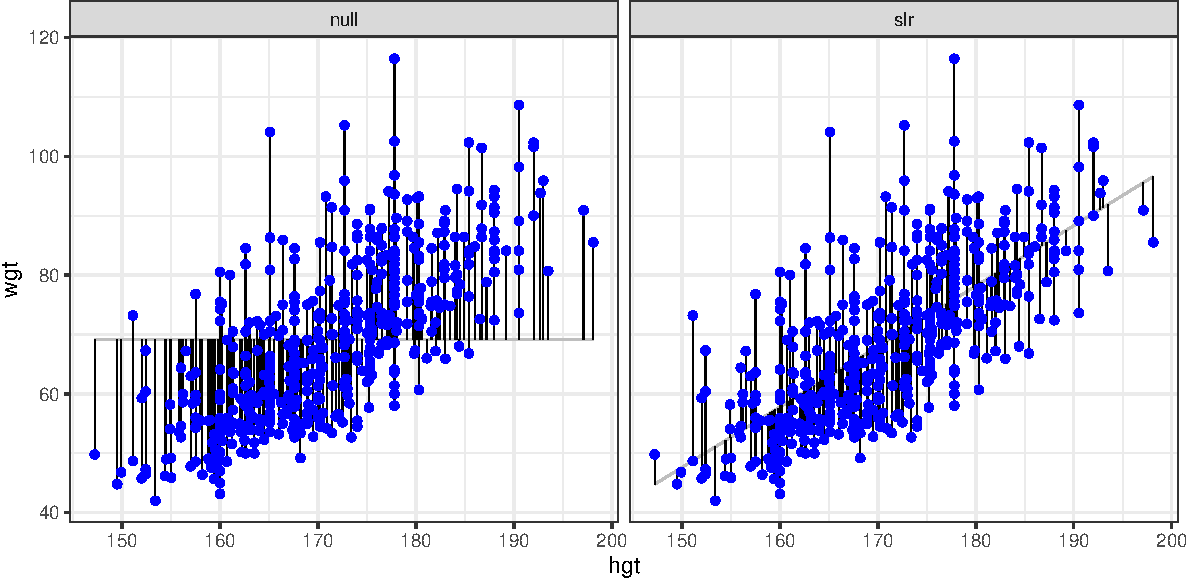
\includegraphics{CorrRegSC_files/figure-latex/fig1-1} 

}

\caption{At left, the model based on overall average weight. At right, the simple linear regression model.}\label{fig:fig1}
\end{figure}

It may be useful to preview these \texttt{augment()}-ed data frames with \texttt{glimpse()}:

\begin{Shaded}
\begin{Highlighting}[]
\KeywordTok{glimpse}\NormalTok{(mod_null)}
\KeywordTok{glimpse}\NormalTok{(mod_hgt)}
\end{Highlighting}
\end{Shaded}

\begin{center}\rule{0.5\linewidth}{0.5pt}\end{center}

\hypertarget{excercise-5}{%
\subsection*{Excercise}\label{excercise-5}}
\addcontentsline{toc}{subsection}{Excercise}

\begin{itemize}
\tightlist
\item
  Compute the sum of the squared residuals (\(SSE\)) for the null model \texttt{mod\_null}.
\end{itemize}

\begin{Shaded}
\begin{Highlighting}[]
\CommentTok{# Compute SSE for null model}
\NormalTok{mod_null }\OperatorTok
\StringTok{  }\KeywordTok{summarize}\NormalTok{(}\DataTypeTok{SSE =} \KeywordTok{var}\NormalTok{(wgt))}
\end{Highlighting}
\end{Shaded}

\begin{verbatim}
# A tibble: 1 x 1
    SSE
  <dbl>
1  178.
\end{verbatim}

\begin{itemize}
\tightlist
\item
  Compute the sum of the squared residuals (\(SSE\)) for the regression model \texttt{mod\_hgt}.
\end{itemize}

\begin{Shaded}
\begin{Highlighting}[]
\CommentTok{# Compute SSE for regression model}
\NormalTok{mod_hgt }\OperatorTok
\StringTok{  }\KeywordTok{summarize}\NormalTok{(}\DataTypeTok{SSE =} \KeywordTok{var}\NormalTok{(.resid))}
\end{Highlighting}
\end{Shaded}

\begin{verbatim}
# A tibble: 1 x 1
    SSE
  <dbl>
1  86.5
\end{verbatim}

\begin{center}\rule{0.5\linewidth}{0.5pt}\end{center}

\hypertarget{leverage}{%
\section{Leverage}\label{leverage}}

The leverage of an observation in a regression model is defined entirely in terms of the distance of that observation from the mean of the explanatory variable. That is, observations close to the mean of the explanatory variable have low leverage, while observations far from the mean of the explanatory variable have high leverage. Points of high leverage may or may not be influential.

The \texttt{augment()} function from the \texttt{broom} package will add the leverage scores (\texttt{.hat}) to a model data frame.

\begin{center}\rule{0.5\linewidth}{0.5pt}\end{center}

\hypertarget{excercise-6}{%
\subsection*{Excercise}\label{excercise-6}}
\addcontentsline{toc}{subsection}{Excercise}

\begin{itemize}
\tightlist
\item
  Use \texttt{augment()} to list the top 6 observations by their leverage scores, in descending order.
\end{itemize}

\begin{Shaded}
\begin{Highlighting}[]
\NormalTok{mod <-}\StringTok{ }\KeywordTok{lm}\NormalTok{(slg }\OperatorTok{~}\StringTok{ }\NormalTok{obp, }\DataTypeTok{data =}\NormalTok{ mlbbat10)}
\CommentTok{# Rank points of high leverage}
\NormalTok{mod }\OperatorTok
\StringTok{  }\KeywordTok{augment}\NormalTok{() }\OperatorTok
\StringTok{  }\KeywordTok{arrange}\NormalTok{(}\KeywordTok{desc}\NormalTok{(.hat)) }\OperatorTok
\StringTok{  }\KeywordTok{head}\NormalTok{()}
\end{Highlighting}
\end{Shaded}

\begin{verbatim}
# A tibble: 6 x 8
    slg   obp .fitted .resid   .hat .sigma .cooksd .std.resid
  <dbl> <dbl>   <dbl>  <dbl>  <dbl>  <dbl>   <dbl>      <dbl>
1     1     1    1.12 -0.120 0.0184  0.137 0.00729     -0.882
2     1     1    1.12 -0.120 0.0184  0.137 0.00729     -0.882
3     1     1    1.12 -0.120 0.0184  0.137 0.00729     -0.882
4     1     1    1.12 -0.120 0.0184  0.137 0.00729     -0.882
5     4     1    1.12  2.88  0.0184  0.108 4.22        21.2  
6     1     1    1.12 -0.120 0.0184  0.137 0.00729     -0.882
\end{verbatim}

\hypertarget{influence}{%
\section{Influence}\label{influence}}

As noted previously, observations of high leverage may or may not be influential. The influence of an observation depends not only on its leverage, but also on the magnitude of its residual. Recall that while leverage only takes into account the explanatory variable (\(\hat{x}\)), the residual depends on the response variable (\(\hat{y}\)) and the fitted value (\(\hat{y}\)).

Influential points are likely to have high leverage and deviate from the general relationship between the two variables. We measure influence using Cook's distance, which incorporates both the leverage and residual of each observation.

\begin{center}\rule{0.5\linewidth}{0.5pt}\end{center}

\begin{itemize}
\tightlist
\item
  Use \texttt{augment()} to list the top 6 observations by their Cook's distance (\texttt{.cooksd}), in descending order.
\end{itemize}

\begin{Shaded}
\begin{Highlighting}[]
\CommentTok{# Rank influential points}
\NormalTok{mod }\OperatorTok
\StringTok{ }\KeywordTok{augment}\NormalTok{() }\OperatorTok
\StringTok{ }\KeywordTok{arrange}\NormalTok{(}\KeywordTok{desc}\NormalTok{(.cooksd)) }\OperatorTok
\StringTok{ }\KeywordTok{head}\NormalTok{()}
\end{Highlighting}
\end{Shaded}

\begin{verbatim}
# A tibble: 6 x 8
    slg   obp .fitted .resid    .hat .sigma .cooksd .std.resid
  <dbl> <dbl>   <dbl>  <dbl>   <dbl>  <dbl>   <dbl>      <dbl>
1  4    1       1.12   2.88  0.0184   0.108   4.22       21.2 
2  0    1       1.12  -1.12  0.0184   0.133   0.638      -8.25
3  0    1       1.12  -1.12  0.0184   0.133   0.638      -8.25
4  0    1       1.12  -1.12  0.0184   0.133   0.638      -8.25
5  0    1       1.12  -1.12  0.0184   0.133   0.638      -8.25
6  1.67 0.667   0.750  0.917 0.00676  0.134   0.154       6.72
\end{verbatim}

\begin{center}\rule{0.5\linewidth}{0.5pt}\end{center}

\hypertarget{removing-outliers}{%
\section{Removing outliers}\label{removing-outliers}}

Observations can be outliers for a number of different reasons. Statisticians must always be careful---and more importantly, transparent---when dealing with outliers. Sometimes, a better model fit can be achieved by simply removing outliers and re-fitting the model. However, one must have strong justification for doing this. A desire to have a higher \(R^2\)is not a good enough reason!

In the \texttt{mlbBat10} data, the outlier with an OBP of 0.550 is Bobby Scales, an infielder who had four hits in 13 at-bats for the Chicago Cubs. Scales also walked seven times, resulting in his unusually high OBP. The justification for removing Scales here is weak. While his performance was unusual, there is nothing to suggest that it is not a valid data point, nor is there a good reason to think that somehow we will learn more about Major League Baseball players by excluding him.

Nevertheless, we can demonstrate how removing him will affect our model.

\begin{center}\rule{0.5\linewidth}{0.5pt}\end{center}

\begin{itemize}
\tightlist
\item
  Use \texttt{filter()} to create a subset of \texttt{mlbBat10} called \texttt{nontrivial\_players} consisting of only those players with at least 10 at-bats and \texttt{OBP} of below 0.500.
\end{itemize}

\begin{Shaded}
\begin{Highlighting}[]
\CommentTok{# Create nontrivial_players}
\NormalTok{nontrivial_players <-}\StringTok{ }\NormalTok{mlbbat10 }\OperatorTok
\StringTok{ }\KeywordTok{filter}\NormalTok{(at_bat }\OperatorTok{>=}\StringTok{ }\DecValTok{10}\NormalTok{, obp }\OperatorTok{<}\StringTok{ }\FloatTok{0.500}\NormalTok{)}
\end{Highlighting}
\end{Shaded}

\begin{itemize}
\tightlist
\item
  Fit the linear model for \texttt{SLG} as a function of \texttt{OBP} for the \texttt{nontrivial\_players}. Save the result as \texttt{mod\_cleaner}.
\end{itemize}

\begin{Shaded}
\begin{Highlighting}[]
\CommentTok{# Fit model to new data}
\NormalTok{mod_cleaner <-}\StringTok{ }\KeywordTok{lm}\NormalTok{(slg }\OperatorTok{~}\StringTok{ }\NormalTok{obp, }\DataTypeTok{data =}\NormalTok{ nontrivial_players)}
\end{Highlighting}
\end{Shaded}

\begin{itemize}
\tightlist
\item
  View the \texttt{summary()} of the new model and compare the slope and \(R^2\) to those of \texttt{mod}, the original model fit to the data on all players.
\end{itemize}

\begin{Shaded}
\begin{Highlighting}[]
\CommentTok{# View model summary}
\KeywordTok{summary}\NormalTok{(mod_cleaner)}
\end{Highlighting}
\end{Shaded}

\begin{verbatim}

Call:
lm(formula = slg ~ obp, data = nontrivial_players)

Residuals:
     Min       1Q   Median       3Q      Max 
-0.31383 -0.04165 -0.00261  0.03992  0.35819 

Coefficients:
             Estimate Std. Error t value Pr(>|t|)    
(Intercept) -0.043326   0.009823  -4.411 1.18e-05 ***
obp          1.345816   0.033012  40.768  < 2e-16 ***
---
Signif. codes:  0 '***' 0.001 '**' 0.01 '*' 0.05 '.' 0.1 ' ' 1

Residual standard error: 0.07011 on 734 degrees of freedom
Multiple R-squared:  0.6937,    Adjusted R-squared:  0.6932 
F-statistic:  1662 on 1 and 734 DF,  p-value: < 2.2e-16
\end{verbatim}

\begin{Shaded}
\begin{Highlighting}[]
\KeywordTok{summary}\NormalTok{(mod_cleaner)}\OperatorTok{$}\NormalTok{r.square}
\end{Highlighting}
\end{Shaded}

\begin{verbatim}
[1] 0.6936567
\end{verbatim}

\begin{Shaded}
\begin{Highlighting}[]
\CommentTok{# Original with all players}
\KeywordTok{summary}\NormalTok{(mod)}\OperatorTok{$}\NormalTok{r.square}
\end{Highlighting}
\end{Shaded}

\begin{verbatim}
[1] 0.6635126
\end{verbatim}

\begin{itemize}
\tightlist
\item
  Visualize the new model with \texttt{ggplot()} and the appropriate \texttt{geom\_*()} functions.
\end{itemize}

\begin{Shaded}
\begin{Highlighting}[]
\KeywordTok{ggplot}\NormalTok{(}\DataTypeTok{data =}\NormalTok{ nontrivial_players, }\KeywordTok{aes}\NormalTok{(}\DataTypeTok{x =}\NormalTok{ obp, }\DataTypeTok{y =}\NormalTok{ slg)) }\OperatorTok{+}
\StringTok{  }\KeywordTok{geom_point}\NormalTok{(}\DataTypeTok{alpha =} \FloatTok{0.33}\NormalTok{) }\OperatorTok{+}\StringTok{ }
\StringTok{  }\KeywordTok{geom_smooth}\NormalTok{(}\DataTypeTok{method =} \StringTok{"lm"}\NormalTok{) }\OperatorTok{+}\StringTok{ }
\StringTok{  }\KeywordTok{theme_bw}\NormalTok{()}
\end{Highlighting}
\end{Shaded}

\begin{verbatim}
`geom_smooth()` using formula 'y ~ x'
\end{verbatim}

\begin{center}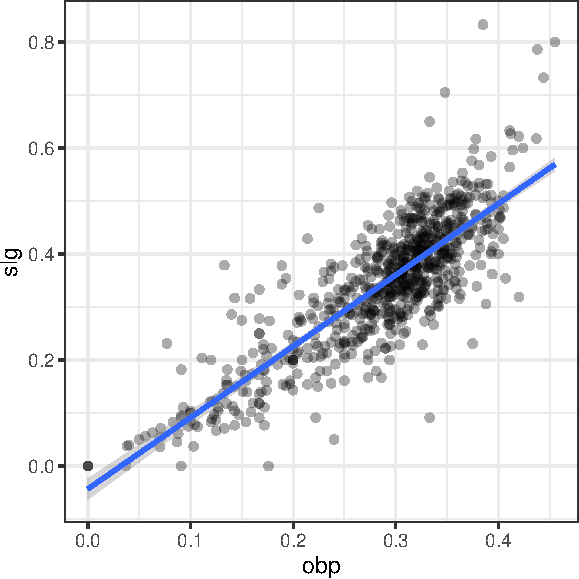
\includegraphics{CorrRegSC_files/figure-latex/unnamed-chunk-72-1} \end{center}

\begin{center}\rule{0.5\linewidth}{0.5pt}\end{center}

\hypertarget{high-leverage-points}{%
\section{High leverage points}\label{high-leverage-points}}

Not all points of high leverage are influential. While the high leverage observation corresponding to Bobby Scales in the previous exercise is influential, the three observations for players with OBP and SLG values of 0 are not influential.

This is because they happen to lie right near the regression anyway. Thus, while their extremely low OBP gives them the power to exert influence over the slope of the regression line, their low SLG prevents them from using it.

\begin{center}\rule{0.5\linewidth}{0.5pt}\end{center}

\begin{itemize}
\tightlist
\item
  The linear model, \texttt{mod}, is available in your workspace. Use a combination of \texttt{augment()}, \texttt{arrange()} with two arguments, and \texttt{head()} to find the top 6 observations with the highest leverage but the lowest Cook's distance.
\end{itemize}

\begin{Shaded}
\begin{Highlighting}[]
\CommentTok{# Rank high leverage points}
\NormalTok{mod }\OperatorTok
\StringTok{ }\KeywordTok{augment}\NormalTok{() }\OperatorTok
\StringTok{ }\KeywordTok{arrange}\NormalTok{(}\KeywordTok{desc}\NormalTok{(.hat), .cooksd) }\OperatorTok
\StringTok{ }\KeywordTok{head}\NormalTok{()}
\end{Highlighting}
\end{Shaded}

\begin{verbatim}
# A tibble: 6 x 8
    slg   obp .fitted .resid   .hat .sigma .cooksd .std.resid
  <dbl> <dbl>   <dbl>  <dbl>  <dbl>  <dbl>   <dbl>      <dbl>
1     1     1    1.12 -0.120 0.0184  0.137 0.00729     -0.882
2     1     1    1.12 -0.120 0.0184  0.137 0.00729     -0.882
3     1     1    1.12 -0.120 0.0184  0.137 0.00729     -0.882
4     1     1    1.12 -0.120 0.0184  0.137 0.00729     -0.882
5     1     1    1.12 -0.120 0.0184  0.137 0.00729     -0.882
6     1     1    1.12 -0.120 0.0184  0.137 0.00729     -0.882
\end{verbatim}

  \bibliography{book.bib,packages.bib}

\end{document}
